\documentclass[11pt,a4paper]{article}

% ======================================================================
%  Clustering, Recovery, and Locality in Algebraic Quantum Field Theory
%  Version 2 (July 2026).  v1: December 16, 2025.
%
%  Summary of changes relative to v1 (see Appendix E for details):
%   1. Corrected the simplified constant: 3/8 -> 7/16 (in the kappa -> infty
%      limit); the v1 statement was inconsistent with its own derivation.
%   2. Added the symplectic-gap hypothesis (f) to Lemma 4.5 / Theorem 4.7,
%      with an explicit counterexample (Remark C.5) showing necessity.
%   3. Fixed the uncertainty-relation convention in Remark 2.6.
%   4. Removed a duplicated passage in Step 5 of the main proof.
%   5. Expanded the proof of Lemma 3.4 (Schur test).
%   6. Added Section 1.3 (relation to prior work) and new references.
% ======================================================================

\usepackage[utf8]{inputenc}
\usepackage[T1]{fontenc}
\usepackage{amsmath,amssymb,amsthm,mathtools}
% Identity operator: uses \mathds{1} if dsfont is available, else bold 1.
\IfFileExists{dsfont.sty}{\usepackage{dsfont}%
  \newcommand{\idm}{\mathds{1}}}{\newcommand{\idm}{\mathbf{1}}}
\usepackage[margin=1.05in]{geometry}
\usepackage{tikz}
\usepackage[colorlinks=true,linkcolor=blue,citecolor=blue,urlcolor=blue]{hyperref}

% ---------- theorem environments ----------
\theoremstyle{plain}
\newtheorem{theorem}{Theorem}[section]
\newtheorem*{theorem*}{Theorem}
\newtheorem*{corollary*}{Corollary}
\newtheorem{lemma}[theorem]{Lemma}
\newtheorem{proposition}[theorem]{Proposition}
\newtheorem{corollary}[theorem]{Corollary}
\newtheorem{conjecture}[theorem]{Conjecture}

\theoremstyle{definition}
\newtheorem{definition}[theorem]{Definition}
\newtheorem{assumption}[theorem]{Assumption}
\newtheorem{example}[theorem]{Example}

\theoremstyle{remark}
\newtheorem{remark}[theorem]{Remark}
\newtheorem*{remark*}{Remark}

% ---------- macros ----------
\newcommand{\Aa}{\mathcal{A}}
\newcommand{\Nn}{\mathcal{N}}
\newcommand{\Mm}{\mathcal{M}}
\newcommand{\Oo}{\mathcal{O}}
\newcommand{\Hh}{\mathcal{H}}
\newcommand{\hh}{\mathfrak{h}}
\newcommand{\R}{\mathbb{R}}
\newcommand{\opnorm}[1]{\left\lVert #1 \right\rVert_{\mathrm{op}}}
\newcommand{\hsnorm}[1]{\left\lVert #1 \right\rVert_{\mathrm{HS}}}
\newcommand{\norm}[1]{\left\lVert #1 \right\rVert}
\newcommand{\Tr}{\operatorname{Tr}}
\newcommand{\rank}{\operatorname{rank}}
\newcommand{\dist}{\operatorname{dist}}
\newcommand{\etavac}{\eta_{\mathrm{vac}}}
\newcommand{\Cvac}{C_{\mathrm{vac}}}
\newcommand{\Neff}{N_{\mathrm{eff}}}
\newcommand{\Ncan}{\Nn_{\mathrm{can}}}
\newcommand{\Ckappa}{C_{\kappa}}
\newcommand{\Cd}{C^{(0)}_{d,\kappa}}
\newcommand{\vc}{\operatorname{vec}}

\title{Clustering, Recovery, and Locality in\\ Algebraic Quantum Field Theory\\[1ex]
\large Quantitative Bounds via Split Inclusions and Modular Theory}
\author{Lluis Eriksson\\ \small Independent Researcher\\ \small \texttt{lluiseriksson@gmail.com}}
\date{July 4, 2026 \quad (v2; v1: December 16, 2025)}

\begin{document}

\maketitle

\begin{abstract}
We prove that exponential clustering of vacuum correlations enables approximate
reconstruction of global quasi-free states from local data in algebraic quantum
field theory. The reconstruction is an explicit Gaussian procedure ---
\emph{conditional reattachment} through the vacuum's regression structure ---
which coincides with the output of the Petz recovery map when the reference state
factorizes across the split, but \emph{not} in general: for a pure reference the
Petz map returns the reference itself for every input, and version~1 of this
paper incorrectly identified the two. For quasi-free states of a massive scalar
field satisfying natural constraints, including a symplectic-gap (mixedness)
condition on the reference state and an admissibility (no-steering) condition on
the split geometry, we prove:
\[
1 - F(\omega, \tilde{\omega}) \;\le\;
\frac{\Cd}{\epsilon^2 \left(1 - \epsilon^{-1}(\etavac + \delta)^2\right)^2}
\cdot \hsnorm{\Delta^{(12)}}^2
\]
where $\Delta^{(12)}$ is the reconstruction error, $\etavac \lesssim e^{-mr}$ is
the vacuum correlation factor, $\delta$ controls cross-correlation perturbations,
and $\Cd = \tfrac{\Ckappa(6+\Ckappa)}{16\min(c_1,c_2)^2}$ with
$\Ckappa = \tfrac{(1+\kappa)^2}{\kappa(\kappa+2)}$ determined by the symplectic gap
$\kappa > 0$. A finite-rank corollary with explicit factor $2n$ recovers physical
intuition. All counterexamples and bounds are verified by an exact truncated-Fock
numerical suite distributed with the paper (Appendix~\ref{app:numerics}).
Applications to holographic reconstruction are discussed.

\medskip
\noindent\textbf{Version 2.} This version makes three corrections to v1: (i) the
reconstruction map of v1's Proposition~2.14 is \emph{not} the Petz map --- its
``marginal preservation'' step fails for correlated references --- and the main
theorem is restated for the reconstruction procedure that the proof actually
controls; (ii) the simplified constant is corrected ($3/8 \to 7/16$ in the
strongly mixed limit); (iii) a symplectic-gap hypothesis is added to the Gaussian
fidelity lemma, shown necessary by an explicit counterexample. See
Appendix~\ref{app:changelog}.
\end{abstract}

\tableofcontents

% ======================================================================
\section{Introduction}

\subsection{The Central Problem}

The interplay between locality, entanglement, and information recovery constitutes a
central theme in modern theoretical physics. The Reeh--Schlieder theorem establishes
long-range vacuum entanglement, yet correlations decay exponentially for massive
theories (clustering).
\begin{center}
\emph{To what extent does clustering enable approximate reconstruction of global
information from local data?}
\end{center}

\subsection{Main Results}

\begin{theorem*}[Clustering--Recovery Bridge; Theorem~\ref{thm:main}]
For quasi-free states satisfying hypotheses (a)--(g) in the regularized framework,
the fidelity between $\omega$ and its conditional-reattachment reconstruction
$\tilde{\omega} = \Lambda_{\Gamma_0}[\omega|_1]$ (Definition~\ref{def:reattach})
satisfies:
\begin{equation}
1 - F(\omega, \tilde{\omega}) \;\le\;
\frac{\Cd}{\epsilon^2 \left(1 - \epsilon^{-1}(\etavac + \delta)^2\right)^2}
\cdot \hsnorm{\Delta^{(12)}}^2
\end{equation}
where:
\begin{itemize}
\item $\Cd = \frac{\Ckappa(6+\Ckappa)}{16 \min(c_1,c_2)^2}$ depends on the vacuum
spectral bounds $c_1, c_2$ of Assumption~\ref{ass:reg} and on the symplectic gap
$\kappa$ of hypothesis (f), through $\Ckappa = \frac{(1+\kappa)^2}{\kappa(\kappa+2)}$
(in the simplified regime of Corollary~\ref{cor:simplified}); in the strongly mixed
limit $\Ckappa \to 1$ one recovers $\Cd \to \frac{7}{16\min(c_1,c_2)^2}$,
\item $\etavac := \opnorm{A_0^{-1/2} X_0 B_0^{-1/2}}$ is the vacuum correlation factor,
\item $\delta := \opnorm{A_0^{-1/2}(X - X_0)B_0^{-1/2}}$ controls cross-correlation
changes.
\end{itemize}
The recovery error decomposes as:
\begin{equation}
\Delta^{(12)} = (X - X_0) - (A - A_0)A_0^{-1}X_0
\end{equation}
\end{theorem*}

\begin{corollary*}[Finite Rank; Corollary~\ref{cor:finiterank}]
If $\rank(\Gamma_\omega - \Gamma_0) \le n$:
\begin{equation}
1 - F(\omega, \tilde{\omega}) \;\le\;
\frac{2\,\Cd \cdot n}{\epsilon^2 \left(1 - \epsilon^{-1}(\etavac + \delta)^2\right)^2}
\cdot \opnorm{\Delta^{(12)}}^2
\end{equation}
with explicit factor $2$ from $\rank(\Delta^{(12)}) \le 2n$.
\end{corollary*}

\begin{remark*}[Corrections relative to v1]
Three corrections. \emph{First and most important}: the state $\tilde{\omega}$
controlled by the proof is \emph{not} the output of the Petz map, contrary to
v1's Proposition~2.14, whose ``marginal preservation'' step fails for correlated
references (Lemma~\ref{lem:petzmarginal}; for a pure reference the Petz map
returns the reference for every input). The theorem is restated for the
conditional-reattachment reconstruction, which is what formula \eqref{eq:petzcov}
describes; it coincides with the Petz output for factorized references and
approaches it in the strongly mixed, weakly correlated regime (exact numerics in
Appendix~\ref{app:numerics}). \emph{Second}: v1 stated the simplified constant as
$\tfrac{3}{8\min(c_1,c_2)^2}$, inconsistent with its own Step~5 (the quartic
remainder contributes $\tfrac{1}{48}$, giving $\tfrac{7}{48}\times 3 =
\tfrac{7}{16}$). \emph{Third}: the Gaussian fidelity lemma requires a
symplectic-gap hypothesis on the reference covariance; without it the quadratic
fidelity bound fails for purity-changing perturbations
(Remark~\ref{rem:counterexample}).
\end{remark*}

\subsection{Relation to Prior Work}\label{sec:related}

The question of when quantum information can be approximately recovered after
restriction to a subalgebra has been studied intensively from the quantum
information side. Petz \cite{Petz86} characterized exact sufficiency of subalgebras
via the recovery map that now bears his name; Fawzi and Renner \cite{FawziRenner15}
proved that small conditional mutual information implies approximate recoverability
in finite dimensions, and Junge, Renner, Sutter, Wilde and Winter \cite{JRSWW18}
constructed universal recovery maps in infinite-dimensional (Type~I) settings.

Closest in spirit to the present work are the results of Faulkner, Hollands, Swingle
and Wang \cite{FHSW22}, and Faulkner and Hollands \cite{FH22}, who proved the
existence of universal recovery channels for inclusions of \emph{general} von Neumann
algebras, with recovery fidelity controlled by the change in relative entropy with
respect to a reference state; see also Junge and LaRacuente \cite{JungeLaRacuente22}
for multivariate trace inequalities and $p$-fidelity beyond tracial settings. Those
results are structural: they hold for arbitrary inclusions but do not by themselves
quantify \emph{how small} the relevant entropy difference is for a given geometry.
The present paper is complementary: we work in a concrete (regularized, quasi-free)
setting where an explicit reconstruction can be analyzed in closed form, and we
trade generality for \emph{explicit constants} tied to the geometry of a split
inclusion, with the collar width $r$ and the mass gap $m$ entering through the
clustering factor $\etavac \lesssim e^{-mr}$. For the exact Petz map of Gaussian
references --- which is a Gaussian channel with an explicit covariance action, but
\emph{not} the reconstruction analyzed here (Section~\ref{sec:petzreattach}) ---
see Lami, Das and Wilde \cite{LamiDasWilde18}. Making contact between the two approaches --- i.e.,
controlling the Faulkner--Hollands--Swingle--Wang entropy difference by clustering
data --- is a promising route toward Conjecture~\ref{conj:general}; see
Section~\ref{sec:strategies}.

On the holographic side, entanglement wedge reconstruction via (twirled) Petz maps
was established by Cotler, Hayden, Penington, Salton, Swingle and Walter
\cite{CotlerEtAl19}, and simplified to the plain Petz map by Chen, Penington and
Salton \cite{ChenPS20}. Our conditional Corollary~\ref{cor:wedge} is a
mass-gap-quantified statement in the same direction. For background on entanglement
measures, the split property, and modular-theoretic constraints in QFT we refer to
Hollands and Sanders \cite{HollandsSanders18} and Lashkari \cite{Lashkari19}.

\subsection{Structure}

Section~\ref{sec:framework} establishes the algebraic framework.
Section~\ref{sec:clustering} develops clustering bounds. Section~\ref{sec:bridge}
contains the main theorem. Section~\ref{sec:conjecture} formulates the general
conjecture. Section~\ref{sec:discussion} presents implications.
Appendix~\ref{app:changelog} lists the changes relative to v1.

% ======================================================================
\section{Algebraic Framework}\label{sec:framework}

\subsection{Haag--Kastler Axioms}

We work in the Haag--Kastler framework \cite{Haag96} on Minkowski spacetime
$\R^{d,1}$ ($d \ge 2$).

\begin{definition}[Haag--Kastler Net]
A net $\Oo \mapsto \Aa(\Oo)$ of von Neumann algebras on $\Hh$ satisfying isotony,
locality, covariance, and the spectrum condition.
\end{definition}

\begin{theorem}[Reeh--Schlieder]
For any region $\Oo$ with non-empty causal complement, the vacuum $\Omega$ is cyclic
and separating for $\Aa(\Oo)$.
\end{theorem}

\subsection{Geometric Setup}

\begin{definition}[Split Configuration]
Double cones $\Oo_1 \Subset \Oo_2$ with collar width
$r := \dist(\partial \Oo_1, \partial \Oo_2) > 0$.
\end{definition}

\begin{figure}[ht]
\centering
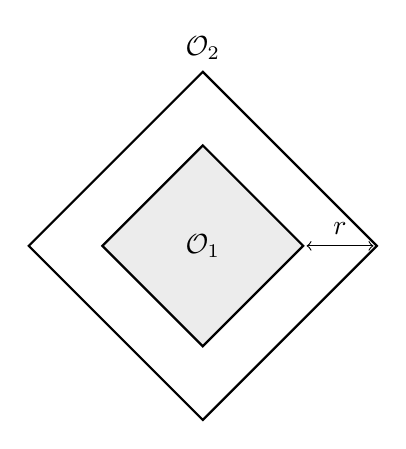
\begin{tikzpicture}[scale=0.85]
  \draw[thick] (0,-2.6) -- (2.6,0) -- (0,2.6) -- (-2.6,0) -- cycle;
  \draw[thick,fill=gray!15] (0,-1.5) -- (1.5,0) -- (0,1.5) -- (-1.5,0) -- cycle;
  \node at (0,0) {$\Oo_1$};
  \node at (0,2.95) {$\Oo_2$};
  \draw[<->] (1.55,0) -- (2.55,0);
  \node[above] at (2.05,0.02) {$r$};
\end{tikzpicture}
\caption{Split configuration: inner region $\Oo_1$, collar width $r$.}
\end{figure}

\subsection{Quasi-Free States}

\begin{definition}[Quasi-Free State]
A state with characteristic function:
\begin{equation}
\omega(W(f)) = \exp\left(-\tfrac{1}{4}\langle f, \Gamma_\omega f\rangle\right)
\end{equation}
\end{definition}

Quasi-free states in the operator-algebraic setting were developed by Araki
\cite{Araki64,Araki70}; see also \cite[Chapter~12]{Holevo11} for CCR quasi-free
(Gaussian) states.

\begin{definition}[Block Decomposition]
For $\hh = \hh_1 \oplus \hh_2$:
\begin{equation}
\Gamma = \begin{pmatrix} A & X \\ X^T & B \end{pmatrix}
\end{equation}
with vacuum blocks $A_0, X_0, B_0$. (All covariance blocks are real matrices in the
quadrature representation; $A$ and $B$ are symmetric.)
\end{definition}

\begin{remark}[CCR covariance convention]\label{rem:convention}
We work with the bosonic CCR algebra in a regularized finite-mode setting. With the
Weyl-operator and characteristic-function conventions of
Appendix~\ref{app:conditional} (Remark~\ref{rem:appconv}), Gaussian states are
parametrized by a real symmetric covariance matrix $\Gamma$ satisfying the
uncertainty condition
\begin{equation}
\Gamma + i\,\Omega \;\ge\; 0,
\end{equation}
where $\Omega$ is the standard symplectic form; in this normalization the one-mode
vacuum has $\Gamma = \idm$ and pure Gaussian states are exactly those whose
symplectic eigenvalues all equal $1$. Under Assumption~\ref{ass:reg}, $\Gamma$ is
strictly positive with $\Gamma \ge c \cdot \idm$ for some $c > 0$.
(In v1 the uncertainty condition was misstated as
$\Gamma + \tfrac{i}{2}\Omega \ge 0$, which belongs to the convention
$\chi = e^{-\frac{1}{2}z^T\Gamma z}$; see Appendix~\ref{app:changelog}.)
\end{remark}

\begin{assumption}[Regularized one-particle framework and uniform lower bounds]
\label{ass:reg}
We work in a regularized setting (e.g., a lattice approximation, finite-mode
truncation, or an explicit UV cutoff) in which the quasi-free covariances are
represented by bounded, strictly positive operators on the one-particle Hilbert
space $\hh = \hh_1 \oplus \hh_2$. In particular, the vacuum blocks satisfy:
\begin{equation}
A_0 \ge c_1 \cdot \idm_{\hh_1}, \qquad B_0 \ge c_2 \cdot \idm_{\hh_2}
\end{equation}
for constants $c_1, c_2 > 0$ depending on the chosen regularization and geometry.
\end{assumption}

\begin{remark}[Verification in regularized settings]
For finite-volume restrictions with smooth boundaries and Dirichlet boundary
conditions, the constants can be estimated from lower bounds on the corresponding
elliptic operator. For a spatial ball of radius $R$ one obtains:
\begin{equation}
c_1, c_2 \ge (m^2 + \pi^2/R^2)^{-1/2}
\end{equation}
For lattice discretizations, $c_1, c_2$ can be bounded in terms of the smallest
eigenvalue of the discrete massive Laplacian on the corresponding finite region. See
Reed--Simon \cite[Theorem~XIII.67]{ReedSimon78} for continuum analogues.
\end{remark}

\begin{remark}[Continuum limit and operator ideal issues]
In continuum AQFT, covariance operators and their blocks may be unbounded, and
conditions such as $\Gamma_\omega - \Gamma_0 \in \mathcal{L}^2(\hh)$ or
$\etavac = \opnorm{A_0^{-1/2} X_0 B_0^{-1/2}} < 1$ require a careful choice of
one-particle space and domains (typically via smearing and Sobolev-type norms).
Accordingly, the present bounds are proved in the regularized framework of
Assumption~\ref{ass:reg}. Extending them to the fully continuum Type~III setting is
left for future work.
\end{remark}

\subsection{The Split Property}

\begin{theorem}[Buchholz--Wichmann--D'Antoni--Longo]
For massive scalar fields satisfying nuclearity \cite{BW86}, the split property
holds: there exists a Type~I factor $\Nn$ with $\Aa \subset \Nn \subset \Mm$.
\end{theorem}

See also Summers \cite{Summers90} for discussion of independence properties of local
algebras related to split inclusions.

\begin{theorem}[Canonical Split Inclusion]\label{thm:canonical}
The canonical split factor $\Ncan$ satisfies:
\begin{enumerate}
\item[(a)] $\Ncan$ is Type~I with $\Aa \subset \Ncan \subset \Mm$
\item[(b)] $\sigma_t^{\omega_0}(\Ncan) = \Ncan$ (modular invariance)
\end{enumerate}
\end{theorem}

\begin{proof}
See Doplicher--Longo \cite[Theorem~4.1]{DoplicherLongo84} and
Buchholz--D'Antoni--Longo \cite[Proposition~3.2]{BDL90}.
\end{proof}

\begin{remark}[Construction-Based Modular Invariance]
For massive fields, modular invariance of $\Ncan$ follows from its construction via
the nuclearity map, not from geometric modular action (which fails for double
cones). The subspace $K_\Xi$ is $\Delta^{it}$-invariant by construction.
\end{remark}

\subsection{Petz Recovery and Conditional Reattachment}\label{sec:petzreattach}

\begin{definition}[Petz Recovery Map]\label{def:petz}
In the regularized tensor product setting $\Mm = B(\Hh_1 \otimes \Hh_2)$ with
$\Nn = B(\Hh_1) \otimes \idm_{\Hh_2}$, let $\rho_0$ be a faithful density
operator on $\Hh_1 \otimes \Hh_2$ and write $\rho_{0,1} := \Tr_2(\rho_0)$ for its
marginal on subsystem~1. The Petz recovery map
$\mathcal{R}_{\rho_0}: \mathcal{S}(\Hh_1) \to \mathcal{S}(\Hh_1 \otimes \Hh_2)$ is:
\begin{equation}\label{eq:petzdef}
\mathcal{R}_{\rho_0}(\sigma_1) := \rho_0^{1/2}\left(\rho_{0,1}^{-1/2}\,\sigma_1\,
\rho_{0,1}^{-1/2} \otimes \idm_{\Hh_2}\right)\rho_0^{1/2}
\end{equation}
where $\sigma_1 \ge 0$ is a density operator on $\Hh_1$ with $\Tr(\sigma_1) = 1$.
\end{definition}

The Petz map always recovers the reference perfectly,
$\mathcal{R}_{\rho_0}(\rho_{0,1}) = \rho_0$, and satisfies $\Tr_2 \circ
\mathcal{R}_{\rho_0} = \mathrm{id}$ \emph{when $\rho_0$ factorizes}. Version~1 of
this paper asserted marginal preservation in general; this is false, and the
failure is maximal for pure references:

\begin{lemma}[Marginal preservation and its failure]\label{lem:petzmarginal}
\leavevmode
\begin{enumerate}
\item[(a)] If $\rho_0 = \rho_{0,1} \otimes \rho_{0,2}$, then
$\mathcal{R}_{\rho_0}(\sigma_1) = \sigma_1 \otimes \rho_{0,2}$ for every
$\sigma_1$; in particular $\Tr_2(\mathcal{R}_{\rho_0}(\sigma_1)) = \sigma_1$.
\item[(b)] If $\rho_0 = |\psi\rangle\langle\psi|$ is pure, then
$\mathcal{R}_{\rho_0}(\sigma_1) = \rho_0$ for \emph{every} $\sigma_1$; in
particular $\Tr_2(\mathcal{R}_{\rho_0}(\sigma_1)) = \rho_{0,1} \ne \sigma_1$
in general. (In part (b) the Petz expression \eqref{eq:petzdef} is understood
on the support of $\rho_0$ --- equivalently with Moore--Penrose inverses, or as
the limit of faithful regularizations $\rho_{0,\varepsilon} =
(1-\varepsilon)|\psi\rangle\langle\psi| + \varepsilon\tau$ with $\tau$ faithful,
under which the conclusion is continuous.)
\end{enumerate}
Consequently $\Tr_2 \circ \mathcal{R}_{\rho_0} \ne \mathrm{id}$ for correlated
references; by Takesaki's theorem, a $\rho_0$-preserving conditional expectation
onto $B(\Hh_1)\otimes\idm$ (whose existence is what marginal preservation would
express) exists precisely when the modular group of $\rho_0$ preserves the
subalgebra, i.e., when $\rho_0$ factorizes.
\end{lemma}

\begin{proof}
(a) With $\rho_0^{1/2} = \rho_{0,1}^{1/2} \otimes \rho_{0,2}^{1/2}$, the inner
factors cancel: $\rho_{0,1}^{1/2}\rho_{0,1}^{-1/2}\sigma_1
\rho_{0,1}^{-1/2}\rho_{0,1}^{1/2} = \sigma_1$.
(b) $\rho_0^{1/2} = |\psi\rangle\langle\psi|$, so
$\mathcal{R}_{\rho_0}(\sigma_1) = |\psi\rangle\langle\psi|\cdot
\langle\psi|(\rho_{0,1}^{-1/2}\sigma_1\rho_{0,1}^{-1/2}\otimes\idm)|\psi\rangle
= \rho_0 \cdot \Tr\!\big(\rho_{0,1}\,\rho_{0,1}^{-1/2}\sigma_1
\rho_{0,1}^{-1/2}\big) = \rho_0$.
\end{proof}

The object that the computations of this paper actually control is the following
explicit reconstruction procedure, which replaces the Petz map throughout.

\begin{definition}[Gaussian conditional reattachment]\label{def:reattach}
Let $\Gamma_0 = \begin{pmatrix} A_0 & X_0 \\ X_0^T & B_0\end{pmatrix}$ be the
vacuum covariance and set the \emph{regression matrix} $W := A_0^{-1}X_0$ and the
\emph{conditional covariance} $C_0 := B_0 - X_0^T A_0^{-1} X_0 \ge 0$ (Schur
complement). The \emph{conditional reattachment} of a centered Gaussian state
$\sigma_1$ with covariance $A$ is the centered Gaussian state
$\tilde{\omega} = \Lambda_{\Gamma_0}[\sigma_1]$ with covariance
\begin{equation}\label{eq:petzcov}
\Gamma_{\tilde{\omega}} = \begin{pmatrix}
A & A W \\
W^T A & C_0 + W^T A W
\end{pmatrix}
= \begin{pmatrix}
A & A A_0^{-1} X_0 \\
X_0^T A_0^{-1} A & B_0 + X_0^T A_0^{-1}(A - A_0)A_0^{-1} X_0
\end{pmatrix},
\end{equation}
whenever $\Gamma_{\tilde{\omega}} + i\Omega \ge 0$ (see
Proposition~\ref{prop:admissible}). Equivalently, $\Lambda_{\Gamma_0}$ is
characterized in the Heisenberg picture by the dual action
\eqref{eq:heisenberg} on Weyl operators (Appendix~\ref{app:conditional}).
\end{definition}

This is the quantum analogue of the classical operation ``keep the observed
marginal on subsystem~1 and reattach subsystem~2 by the reference's conditional
distribution (regression)''; the second expression in \eqref{eq:petzcov} is the
formula that v1 attributed to the Petz map.

\begin{remark}[Reattachment is a reconstruction, not a channel]\label{rem:notchannel}
The assignment $\sigma_1 \mapsto \Lambda_{\Gamma_0}[\sigma_1]$ is a well-defined
map from admissible Gaussian states to Gaussian states, but for $X_0 \neq 0$ it is
\emph{not} the restriction of any completely positive channel: a Gaussian channel
with $X$-matrix $\binom{\idm}{W^T}$ and noise $Y = \mathrm{diag}(0, C_0)$ must
satisfy $Y + i(\Omega - X\Omega_1 X^T) \ge 0$ \cite[Chapter~12]{Holevo11}, whose
$(1,1)$ block vanishes while the off-diagonal block equals $-i\Omega_1 W \ne 0$
--- a positive semidefinite matrix with a vanishing diagonal block has vanishing
off-diagonal blocks, so complete positivity fails. Physically this is a
no-broadcasting obstruction: no channel can correlate its output with fresh
degrees of freedom conditionally on the input while leaving the input marginal
untouched. Accordingly, Theorem~\ref{thm:main} is a statement about the accuracy
of an explicitly computable \emph{state reconstruction} from local data, not
about a physical recovery operation; the true Petz map \emph{is} a Gaussian
channel for Gaussian references \cite{LamiDasWilde18}, agrees with
$\Lambda_{\Gamma_0}$ when $X_0 = 0$ (Lemma~\ref{lem:petzmarginal}(a) and
Lemma~\ref{lem:heisenberg}), and approaches it in the strongly-mixed, weakly
correlated regime (Appendix~\ref{app:numerics}).
\end{remark}

\begin{proposition}[Admissibility of the reattachment]\label{prop:admissible}
Assume $\nu_{\min}(A) \ge 1 + \kappa_1$ and $\nu_{\min}(B_0) \ge 1 + \nu_0$ for
some $\kappa_1, \nu_0 > 0$ (symplectic gaps of the blocks), and let
$\gamma_1 := \tfrac{\kappa_1}{1+\kappa_1}\lambda_{\min}(A)$,
$\gamma_2 := \tfrac{\nu_0}{1+\nu_0}\, c_2$. If
\begin{equation}\label{eq:admissible}
\Cvac^2\,\etavac^2 \;\le\; \gamma_1\left(\gamma_2 - \etavac^2\opnorm{B_0}
- \Cvac^2\etavac^2\right),
\end{equation}
then $\Gamma_{\tilde{\omega}} + i\Omega \ge 0$, i.e., $\tilde{\omega}$ is a valid
Gaussian state. In particular, since $\etavac \le C_d K_\nu(mr)$
(Lemma~\ref{lem:vacbound}), there is $r_1 > 0$ such that \eqref{eq:admissible}
holds for all $r \ge r_1$.
\end{proposition}

\begin{proof}
Write $S := \begin{pmatrix} \idm & 0 \\ W^T & \idm \end{pmatrix}$, so that
$\Gamma_{\tilde{\omega}} = S\,\mathrm{diag}(A, C_0)\,S^T$. Congruence by $S$
preserves positive semidefiniteness, so $\Gamma_{\tilde{\omega}} + i\Omega \ge 0$
is equivalent to $N := \mathrm{diag}(A, C_0) + i\,S^{-1}\Omega S^{-T} \ge 0$.
A direct computation gives
\begin{equation}
S^{-1}\Omega S^{-T} =
\begin{pmatrix} \Omega_1 & -\Omega_1 W \\ -W^T\Omega_1 & \Omega_2 + W^T\Omega_1 W
\end{pmatrix},
\qquad
N = \begin{pmatrix} A + i\Omega_1 & -i\Omega_1 W \\
-iW^T\Omega_1 & C_0 + i\Omega_2 + iW^T\Omega_1 W \end{pmatrix}.
\end{equation}
For the diagonal blocks: $\nu_{\min}(A) \ge 1+\kappa_1$ is equivalent to
$\opnorm{A^{-1/2}\Omega_1 A^{-1/2}} \le (1+\kappa_1)^{-1}$, hence
$A + i\Omega_1 \ge \big(1 - \tfrac{1}{1+\kappa_1}\big)A \ge \gamma_1 \idm$;
similarly $B_0 + i\Omega_2 \ge \tfrac{\nu_0}{1+\nu_0}B_0 \ge \gamma_2\idm$, and
since $X_0^T A_0^{-1} X_0 = B_0^{1/2}Y^TYB_0^{1/2}$ with
$Y = A_0^{-1/2}X_0B_0^{-1/2}$,
\begin{equation}
C_0 + i\Omega_2 + iW^T\Omega_1 W \;\ge\;
\big(\gamma_2 - \etavac^2\opnorm{B_0} - \opnorm{W}^2\big)\idm,
\qquad \opnorm{W} \le \Cvac\etavac
\end{equation}
by Lemma~\ref{lem:crossbound}. For the off-diagonal block,
$\opnorm{\Omega_1 W} = \opnorm{W} \le \Cvac\etavac$. A Hermitian block matrix
$\begin{pmatrix} P & Z \\ Z^\dagger & Q\end{pmatrix}$ with $P \ge \gamma_1\idm$,
$Q \ge \gamma_2'\idm$ and $\opnorm{Z}^2 \le \gamma_1\gamma_2'$ is positive
semidefinite (Schur complement); applying this with
$\gamma_2' = \gamma_2 - \etavac^2\opnorm{B_0} - \Cvac^2\etavac^2$ and
$\opnorm{Z} \le \Cvac\etavac$ gives the claim under \eqref{eq:admissible}.
\end{proof}

\begin{remark}[Steering]\label{rem:steering}
Condition \eqref{eq:admissible} can genuinely fail at small collar width: if the
reference $\rho_0$ is strongly entangled across the split (e.g., two-mode squeezed
with large squeezing and low temperature), the conditional covariance $C_0$
violates $C_0 + i\Omega_2 \ge 0$ --- this is exactly Gaussian steerability of
subsystem~2 by measurements on subsystem~1 --- and no Gaussian state has the
covariance \eqref{eq:petzcov}. The exponential decay of $\etavac$ guarantees
admissibility for $mr$ large, which is the regime of interest throughout.
\end{remark}

% ======================================================================
\section{Exponential Clustering for Massive Fields}\label{sec:clustering}

This section establishes quantitative bounds on correlation decay.

\subsection{The Vacuum Two-Point Function}

\begin{theorem}[Vacuum Clustering]\label{thm:clustering}
For the massive scalar field ($m > 0$) on $\R^{d,1}$, the equal-time two-point
function at spatial separation $s$ satisfies:
\begin{equation}\label{eq:twopoint}
|\omega_0(\phi(x)\phi(y))| = \frac{1}{(2\pi)^{(d-1)/2}} \frac{K_\nu(ms)}{s^{\nu}}
\end{equation}
where $\nu = (d-2)/2$ and $K_\nu$ is the modified Bessel function of the second kind.
\end{theorem}

\begin{corollary}[Bessel Asymptotics]\label{cor:bessel}
For $ms \gg 1$:
\begin{equation}
K_\nu(ms) \sim \sqrt{\frac{\pi}{2ms}}\, e^{-ms}
\end{equation}
Thus correlations decay as $s^{-(d-1)/2} e^{-ms}$. See
\cite[\S10.40]{NIST} for the uniform asymptotic expansions used here and in
Appendix~\ref{app:bessel}.
\end{corollary}

\subsection{The Vacuum Correlation Factor}

\begin{definition}[Vacuum Correlation Factor]
For a split configuration with collar width $r$:
\begin{equation}
\etavac := \opnorm{A_0^{-1/2} X_0 B_0^{-1/2}}
\end{equation}
\end{definition}

\begin{lemma}[Vacuum Correlation Bound]\label{lem:vacbound}
For the massive scalar field in the regularized framework of
Assumption~\ref{ass:reg}, there exist constants $C_d' = C'(d, m, \Oo_1, \Oo_2) > 0$
and $r_0 > 0$ such that for $r \ge r_0$:
\begin{equation}
\etavac \;\le\; C_d \cdot K_\nu(mr) \;<\; \frac{1}{2},
\qquad C_d := (c_1 c_2)^{-1/2}\, C_d'.
\end{equation}
\end{lemma}

\begin{proof}
\emph{Step 1 (kernel bound).} In the regularized setting the off-diagonal block
$X_0$ acts with integral kernel $G_0(x,y) = \omega_0(\phi(x)\phi(y))$ restricted to
$x \in \Sigma_1$, $y \in \Sigma_2$, where $\Sigma_1 \subset \Oo_1$ and $\Sigma_2$
lies at spatial distance $\ge r$ from $\Sigma_1$. By
Theorem~\ref{thm:clustering},
\begin{equation}
|G_0(x,y)| \;\le\; \frac{1}{(2\pi)^{(d-1)/2}}\,
\frac{K_\nu(m|x-y|)}{|x-y|^{\nu}}, \qquad |x-y| \ge r.
\end{equation}

\emph{Step 2 (Schur test).} The Schur test gives
$\opnorm{X_0} \le \sqrt{S_1 S_2}$ with
$S_1 = \sup_{x \in \Sigma_1} \int_{\Sigma_2} |G_0(x,y)|\,dy$ and
$S_2 = \sup_{y \in \Sigma_2} \int_{\Sigma_1} |G_0(x,y)|\,dx$. Passing to spherical
coordinates around $x$ (resp.\ $y$) and using that the integrand is supported on
$|x - y| \ge r$:
\begin{equation}
S_1, S_2 \;\le\; \frac{\omega_{d-2}}{(2\pi)^{(d-1)/2}}
\int_r^{\infty} \frac{K_\nu(ms)}{s^{\nu}}\, s^{d-2}\, ds,
\end{equation}
where $\omega_{d-2}$ is the volume of the unit $(d-2)$-sphere. Since
$K_\nu(z) \le \sqrt{\pi/(2z)}\,e^{-z}\,(1 + O(z^{-1}))$ uniformly for
$z \ge \max(1, \nu^2)$ (Appendix~\ref{app:bessel}), the integral is bounded, for
$mr \ge \max(1,\nu^2)$, by $C''(d,m)\, r^{d-2-\nu}\, e^{-mr}
\le C_d'\, K_\nu(mr)$ after absorbing polynomial factors into $C_d'$ for
$r \ge r_0$. Hence $\opnorm{X_0} \le C_d' \cdot K_\nu(mr)$.

\emph{Step 3 (spectral bounds).} By Assumption~\ref{ass:reg}:
$\opnorm{A_0^{-1/2}} \le c_1^{-1/2}$ and $\opnorm{B_0^{-1/2}} \le c_2^{-1/2}$.

\emph{Step 4 (conclusion).} Combining:
$\etavac \le (c_1 c_2)^{-1/2}\, C_d'\, K_\nu(mr) = C_d\, K_\nu(mr)$. Since
$K_\nu(mr) \to 0$ exponentially as $r \to \infty$, we may enlarge $r_0$ so that the
right-hand side is $< 1/2$ for all $r \ge r_0$.
\end{proof}

\subsection{Auxiliary Constant}

\begin{definition}[Vacuum Amplification Constant]
Define:
\begin{equation}
\Cvac := c_1^{-1/2} \sqrt{\opnorm{B_0}}
\end{equation}
where $c_1$ is from Assumption~\ref{ass:reg}.
\end{definition}

\begin{lemma}[Cross-Correlation Bound]\label{lem:crossbound}
The operator $A_0^{-1} X_0$ satisfies:
\begin{equation}
\opnorm{A_0^{-1} X_0} \le \Cvac \cdot \etavac
\end{equation}
\end{lemma}

\begin{proof}
\begin{align}
\opnorm{A_0^{-1} X_0}
&\le \opnorm{A_0^{-1/2}} \cdot \opnorm{A_0^{-1/2} X_0} \\
&\le c_1^{-1/2} \cdot \opnorm{A_0^{-1/2} X_0 B_0^{-1/2}} \cdot \opnorm{B_0^{1/2}} \\
&= c_1^{-1/2} \cdot \etavac \cdot \sqrt{\opnorm{B_0}} = \Cvac \cdot \etavac
\qedhere
\end{align}
\end{proof}

% ======================================================================
\section{The Clustering--Recovery Bridge}\label{sec:bridge}

This section contains the main result with complete proof.

\subsection{State Class and Hypotheses}

\begin{definition}[Partial Local Excitation]
A quasi-free state $\omega$ is a \emph{partial local excitation} if
$\Gamma_\omega^{(22)} = \Gamma_0^{(22)}$ (i.e., $B = B_0$).
\end{definition}

\begin{definition}[Effective Excitation Number]
\begin{equation}
\Neff(\omega) := \hsnorm{\Gamma_\omega - \Gamma_0}^2
\end{equation}
\end{definition}

\begin{definition}[Cross-Correlation Perturbation]
\begin{equation}
\delta_X := \opnorm{A_0^{-1/2}(X - X_0)B_0^{-1/2}}
\end{equation}
\end{definition}

\begin{definition}[Symplectic Gap]\label{def:sympgap}
A covariance matrix $\Gamma$ has \emph{symplectic gap} $\kappa > 0$ if all its
symplectic eigenvalues satisfy $\nu_j(\Gamma) \ge 1 + \kappa$ (equivalently,
$\Gamma \ge (1+\kappa)\,|i\Omega|$ in the sense that
$\Gamma + (1+\kappa)\, i\Omega \ge 0$). We set
\begin{equation}
\Ckappa := \frac{(1+\kappa)^2}{(1+\kappa)^2 - 1} = \frac{(1+\kappa)^2}{\kappa(\kappa+2)},
\end{equation}
so that $\Ckappa \downarrow 1$ as $\kappa \to \infty$ and $\Ckappa \to \infty$ as
$\kappa \downarrow 0$ (approach to purity).
\end{definition}

\begin{remark}[Consequence of hypothesis (c)]\label{rem:hypc}
The condition $\opnorm{A_0^{-1/2}(A - A_0)A_0^{-1/2}} \le 1 - \epsilon$ implies that
the self-adjoint operator $A_0^{-1/2}(A - A_0)A_0^{-1/2}$ has spectrum in
$[-(1-\epsilon), 1-\epsilon]$. In particular
$A_0^{-1/2}(A - A_0)A_0^{-1/2} \ge -(1-\epsilon)\idm$, hence
$A_0^{-1/2} A A_0^{-1/2} \ge \epsilon\, \idm$, which gives
$A \ge \epsilon A_0$. This inequality is used in Step~4 of the proof of
Theorem~\ref{thm:main}.
\end{remark}

\subsection{Supporting Lemmas}

\begin{lemma}[Gaussian Fidelity Bound]\label{lem:fidelity}
Let $\omega_1, \omega_2$ be quasi-free states with covariances $\Gamma_1, \Gamma_2$
satisfying:
\begin{enumerate}
\item[(i)] $\Gamma_1, \Gamma_2 \ge c \cdot \idm$ for some $c > 0$,
\item[(ii)] $K := \Gamma_1^{-1/2}(\Gamma_1 - \Gamma_2)\Gamma_1^{-1/2}
\in \mathcal{L}^2(\hh)$ (Hilbert--Schmidt class; see
\cite[Chapter~2]{Simon05}),
\item[(iii)] $\opnorm{K} \le 1/2$,
\item[(iv)] $\Gamma_1$ has symplectic gap $\kappa > 0$
(Definition~\ref{def:sympgap}).
\end{enumerate}
Then:
\begin{equation}\label{eq:fidelitybound}
1 - F(\omega_1, \omega_2) \;\le\; \frac{\Ckappa}{8} \hsnorm{K}^2
+ \frac{\Ckappa^2}{48} \hsnorm{K}^4
\end{equation}
Moreover, if either $\Ckappa \le 2$ and $\hsnorm{K} \le 1$, or more generally
$\Ckappa\hsnorm{K}^2 \le 2$, then
\begin{equation}
1 - F(\omega_1, \omega_2) \;\le\; \frac{\Ckappa}{6} \hsnorm{K}^2.
\end{equation}
In all applications below we use the safe two-term bound
\eqref{eq:fidelitybound}; the $\Ckappa/6$ form is quoted only under its
stated smallness condition (cf.\ Appendix~\ref{app:fidelity}).
\end{lemma}

\begin{proof}
See Appendix~\ref{app:fidelity} for the derivation from the exact Gaussian fidelity
formula of Banchi--Braunstein--Pirandola \cite{BanchiBP15}. Hypothesis (iv) is
necessary: without a symplectic gap the quadratic bound fails for perturbations that
increase mixedness (Remark~\ref{rem:counterexample}).
\end{proof}

\begin{lemma}[Block Inversion Bound]\label{lem:blockinv}
Let $\Gamma = \begin{pmatrix} A & X \\ X^T & B \end{pmatrix}$ with:
\begin{enumerate}
\item[(i)] $A \ge \epsilon_A \cdot \idm$, $B \ge \epsilon_B \cdot \idm$,
\item[(ii)] $\eta := \opnorm{A^{-1/2} X B^{-1/2}} < 1$.
\end{enumerate}
Then:
\begin{equation}
\opnorm{\Gamma^{-1}} \le \frac{1}{(1 - \eta^2)\min(\epsilon_A, \epsilon_B)}
\end{equation}
\end{lemma}

\begin{proof}
The Schur complement $S = A - X B^{-1} X^T = A^{1/2}(\idm - K K^T)A^{1/2}$
where $K = A^{-1/2} X B^{-1/2}$. Since $\opnorm{K K^T} = \eta^2 < 1$:
\begin{equation}
S \ge (1 - \eta^2) A \ge (1 - \eta^2)\epsilon_A \cdot \idm
\end{equation}
The block inversion formula then gives the stated bound.
\end{proof}

\subsection{Main Theorem}

\begin{theorem}[Clustering--Recovery Bridge]\label{thm:main}
Let $\omega_0$ denote the vacuum quasi-free state in the regularized framework of
Assumption~\ref{ass:reg}, modeling a massive scalar field ($m > 0$). Let
$\Oo_1 \Subset \Oo_2$ with collar width $r > 0$.

Let $\omega$ be a quasi-free state and let
$\tilde{\omega} := \Lambda_{\Gamma_0}[\omega|_1]$ be the conditional-reattachment
reconstruction (Definition~\ref{def:reattach}) built from the restriction of
$\omega$ to subsystem~1 and the vacuum regression structure. Assume $\omega$
satisfies:
\begin{enumerate}
\item[(a)] (\emph{Partial local excitation}) $B = B_0$,
\item[(b)] (\emph{Finite excitation}) $\Neff(\omega) < \infty$,
\item[(c)] (\emph{Perturbative regime})
$\opnorm{A_0^{-1/2}(A - A_0)A_0^{-1/2}} \le 1 - \epsilon$ for some
$\epsilon \in (0,1)$,
\item[(d)] (\emph{Cross-correlation control}) $\delta_X \le \delta$ for some
$\delta \in (0,1)$ with
\begin{equation}\label{eq:hypd}
\epsilon^{-1/2}(\etavac + \delta) < 1,
\end{equation}
\item[(e)] (\emph{Fidelity regime}) With
$K := \Gamma_\omega^{-1/2}(\Gamma_\omega - \Gamma_{\tilde{\omega}})
\Gamma_\omega^{-1/2}$, we have $\opnorm{K} \le \tfrac{1}{2}$,
\item[(f)] (\emph{Symplectic gap}) $\Gamma_\omega$ has symplectic gap $\kappa > 0$
(Definition~\ref{def:sympgap}),
\item[(g)] (\emph{Admissibility}) $\Gamma_{\tilde{\omega}} + i\Omega \ge 0$, for
which Proposition~\ref{prop:admissible} gives an explicit sufficient condition,
automatic for $mr$ large.
\end{enumerate}
(Note that \eqref{eq:hypd} with $\epsilon < 1$ already implies $\etavac < 1$, so no
separate assumption is needed.)

Define:
\begin{equation}
\eta_\omega := \opnorm{A^{-1/2} X B_0^{-1/2}}
\end{equation}
Then the reconstructed state $\tilde{\omega}$ satisfies:
\begin{equation}\label{eq:mainbound}
1 - F(\omega, \tilde{\omega}) \;\le\;
\frac{\Cd}{\epsilon^2\left(1 - \epsilon^{-1}(\etavac + \delta)^2\right)^2}
\cdot \hsnorm{\Delta^{(12)}}^2
\end{equation}
where:
\begin{itemize}
\item $\Delta^{(12)} := X - A A_0^{-1} X_0$ is the \emph{reconstruction error},
\item the simplified constant
\begin{equation}\label{eq:constant}
\Cd := \frac{\Ckappa\,(6 + \Ckappa)}{16\,\min(c_1, c_2)^2}
\end{equation}
applies under the additional hypotheses of Corollary~\ref{cor:simplified}. In the
strongly mixed limit $\kappa \to \infty$ (i.e., $\Ckappa \to 1$) this reduces to
$\frac{7}{16\min(c_1,c_2)^2}$.
\end{itemize}
Moreover, the recovery error satisfies:
\begin{equation}\label{eq:recerror}
\hsnorm{\Delta^{(12)}} \le (1 + \Cvac \cdot \etavac)\sqrt{\Neff(\omega)}
\end{equation}
where $\Cvac = c_1^{-1/2}\sqrt{\opnorm{B_0}}$.
\end{theorem}

\begin{proof}
We proceed in five steps.

\emph{Step 1: Covariance of the reconstructed state.} By
Definition~\ref{def:reattach} (whose blocks are derived in
Appendix~\ref{app:conditional}), using hypothesis (g):
\begin{equation}
\Gamma_{\tilde{\omega}} = \begin{pmatrix}
A & A A_0^{-1} X_0 \\
X_0^T A_0^{-1} A & B_0 + X_0^T A_0^{-1}(A - A_0)A_0^{-1} X_0
\end{pmatrix}
\end{equation}
The covariance error $\Delta\Gamma := \Gamma_\omega - \Gamma_{\tilde{\omega}}$ has
blocks:
\begin{align}
\Delta^{(11)} &= 0 \\
\Delta^{(12)} &= X - A A_0^{-1} X_0 \\
\Delta^{(22)} &= -X_0^T A_0^{-1}(A - A_0)A_0^{-1} X_0
\end{align}

\emph{Step 2: Decomposition of $\Delta^{(12)}$.}
\begin{align}
\Delta^{(12)} &= X - A A_0^{-1} X_0 \\
&= (X - X_0) + X_0 - A A_0^{-1} X_0 \\
&= (X - X_0) - (A - A_0)A_0^{-1} X_0
\end{align}

\emph{Step 3: Hilbert--Schmidt bound on $\Delta^{(12)}$.} By the triangle
inequality:
\begin{equation}
\hsnorm{\Delta^{(12)}} \le \hsnorm{X - X_0} + \hsnorm{(A - A_0)A_0^{-1} X_0}
\end{equation}
For the first term, since $X - X_0$ is a block of $\Gamma_\omega - \Gamma_0$:
\begin{equation}
\hsnorm{X - X_0} \le \hsnorm{\Gamma_\omega - \Gamma_0} = \sqrt{\Neff(\omega)}
\end{equation}
For the second term, using $\hsnorm{TS} \le \hsnorm{T}\opnorm{S}$:
\begin{align}
\hsnorm{(A - A_0)A_0^{-1} X_0}
&\le \hsnorm{A - A_0} \cdot \opnorm{A_0^{-1} X_0} \\
&\le \sqrt{\Neff(\omega)} \cdot \Cvac \cdot \etavac
\end{align}
where we used Lemma~\ref{lem:crossbound}. Combining:
\begin{equation}\label{eq:step3}
\hsnorm{\Delta^{(12)}} \le (1 + \Cvac \cdot \etavac)\sqrt{\Neff(\omega)}
\end{equation}

\emph{Step 4: Control of $\eta_\omega$ and $\opnorm{\Gamma_\omega^{-1}}$.} We bound
$\eta_\omega = \opnorm{A^{-1/2} X B_0^{-1/2}}$ using the triangle inequality:
\begin{equation}
\eta_\omega \le \opnorm{A^{-1/2} X_0 B_0^{-1/2}}
+ \opnorm{A^{-1/2}(X - X_0)B_0^{-1/2}}
\end{equation}
\emph{First term:} using $A \ge \epsilon A_0$ from hypothesis (c) and
Remark~\ref{rem:hypc}:
\begin{equation}
\opnorm{A^{-1/2} X_0 B_0^{-1/2}}
\le \opnorm{A^{-1/2} A_0^{1/2}} \cdot \opnorm{A_0^{-1/2} X_0 B_0^{-1/2}}
\le \epsilon^{-1/2} \cdot \etavac
\end{equation}
\emph{Second term:} similarly,
\begin{equation}
\opnorm{A^{-1/2}(X - X_0)B_0^{-1/2}}
\le \opnorm{A^{-1/2} A_0^{1/2}} \cdot \opnorm{A_0^{-1/2}(X - X_0)B_0^{-1/2}}
\le \epsilon^{-1/2} \cdot \delta_X \le \epsilon^{-1/2} \delta
\end{equation}
Combining:
\begin{equation}
\eta_\omega \le \epsilon^{-1/2}(\etavac + \delta) < 1
\end{equation}
by hypothesis (d). By Lemma~\ref{lem:blockinv} with $\epsilon_A = \epsilon c_1$ and
$\epsilon_B = c_2$:
\begin{equation}
\opnorm{\Gamma_\omega^{-1}} \le
\frac{1}{(1 - \eta_\omega^2)\min(\epsilon c_1, c_2)}
\end{equation}
Since $\eta_\omega^2 \le \epsilon^{-1}(\etavac + \delta)^2$:
\begin{equation}\label{eq:gammainv}
\opnorm{\Gamma_\omega^{-1}} \le
\frac{1}{\left(1 - \epsilon^{-1}(\etavac + \delta)^2\right)\min(\epsilon c_1, c_2)}
\end{equation}

\emph{Step 5: Apply fidelity bound.} Define
$K := \Gamma_\omega^{-1/2}\,\Delta\Gamma\,\Gamma_\omega^{-1/2}$. By hypothesis (e),
$\opnorm{K} \le \tfrac{1}{2}$; by hypothesis (f), $\Gamma_\omega$ has symplectic gap
$\kappa$. By Lemma~\ref{lem:fidelity}:
\begin{equation}\label{eq:step5start}
1 - F(\omega, \tilde{\omega}) \le \frac{\Ckappa}{8}\hsnorm{K}^2
+ \frac{\Ckappa^2}{48}\hsnorm{K}^4
\end{equation}
Using $\hsnorm{K} \le \opnorm{\Gamma_\omega^{-1}}\hsnorm{\Delta\Gamma}$:
\begin{equation}\label{eq:step5two}
1 - F(\omega, \tilde{\omega}) \le
\frac{\Ckappa}{8}\opnorm{\Gamma_\omega^{-1}}^2\hsnorm{\Delta\Gamma}^2
+ \frac{\Ckappa^2}{48}\opnorm{\Gamma_\omega^{-1}}^4\hsnorm{\Delta\Gamma}^4
\end{equation}
Since $\Delta^{(11)} = 0$:
\begin{equation}
\hsnorm{\Delta\Gamma}^2 = 2\hsnorm{\Delta^{(12)}}^2 + \hsnorm{\Delta^{(22)}}^2
\end{equation}
We bound $\hsnorm{\Delta^{(22)}}$ explicitly. From Step~1:
\begin{equation}
\Delta^{(22)} = -X_0^T A_0^{-1}(A - A_0)A_0^{-1} X_0
\end{equation}
Using $\hsnorm{TSU} \le \opnorm{T}\hsnorm{S}\opnorm{U}$ and
Lemma~\ref{lem:crossbound}:
\begin{equation}
\hsnorm{\Delta^{(22)}} \le (\Cvac \cdot \etavac)^2 \cdot \sqrt{\Neff}
\end{equation}
Therefore:
\begin{equation}\label{eq:deltatot}
\hsnorm{\Delta\Gamma}^2 \le 2\hsnorm{\Delta^{(12)}}^2 + (\Cvac \etavac)^4 \Neff
\end{equation}
This yields the general bound \eqref{eq:step5two}--\eqref{eq:deltatot}. To obtain
the simplified form \eqref{eq:mainbound} with the constant \eqref{eq:constant}, we
impose the additional conditions of Corollary~\ref{cor:simplified}:
\begin{itemize}
\item Under condition (i) of Corollary~\ref{cor:simplified},
$(\Cvac\etavac)^4 \Neff \le \hsnorm{\Delta^{(12)}}^2$, so by \eqref{eq:deltatot}
\begin{equation}\label{eq:three}
\hsnorm{\Delta\Gamma}^2 \le 3\hsnorm{\Delta^{(12)}}^2.
\end{equation}
\item Under condition (ii) of Corollary~\ref{cor:simplified},
$\opnorm{\Gamma_\omega^{-1}}\hsnorm{\Delta\Gamma} \le 1$, hence
$\hsnorm{K} \le 1$ and the quartic term in \eqref{eq:step5two} satisfies
$\frac{\Ckappa^2}{48}\hsnorm{K}^4 \le \frac{\Ckappa^2}{48}\hsnorm{K}^2$, so
\begin{equation}\label{eq:absorb}
1 - F(\omega, \tilde{\omega}) \le
\left(\frac{\Ckappa}{8} + \frac{\Ckappa^2}{48}\right)
\opnorm{\Gamma_\omega^{-1}}^2 \hsnorm{\Delta\Gamma}^2
= \frac{\Ckappa(6 + \Ckappa)}{48}
\opnorm{\Gamma_\omega^{-1}}^2 \hsnorm{\Delta\Gamma}^2.
\end{equation}
\end{itemize}
Finally, using \eqref{eq:gammainv} and
$\min(\epsilon c_1, c_2)^2 \ge \epsilon^2 \min(c_1, c_2)^2$ (valid since
$\epsilon < 1$):
\begin{equation}
\opnorm{\Gamma_\omega^{-1}}^2 \le
\frac{1}{\epsilon^2 \min(c_1,c_2)^2
\left(1 - \epsilon^{-1}(\etavac + \delta)^2\right)^2}.
\end{equation}
Combining this with \eqref{eq:three} and \eqref{eq:absorb} yields
\begin{equation}
1 - F(\omega, \tilde{\omega}) \le
\frac{\Cd}{\epsilon^2\left(1 - \epsilon^{-1}(\etavac + \delta)^2\right)^2}
\cdot \hsnorm{\Delta^{(12)}}^2,
\qquad
\Cd = \frac{\Ckappa(6+\Ckappa)}{16\,\min(c_1,c_2)^2},
\end{equation}
since $3 \times \frac{\Ckappa(6+\Ckappa)}{48} = \frac{\Ckappa(6+\Ckappa)}{16}$. The
conditions (i)--(ii) are satisfied for localized excitations when $mr \gg 1$, as
stated in Corollary~\ref{cor:simplified}.
\end{proof}

\begin{remark}[On the v1 constant]\label{rem:v1constant}
In the limit $\Ckappa \to 1$ the constant is
$\frac{7}{16\min(c_1,c_2)^2}$. Version~1 of this paper stated
$\frac{3}{8\min(c_1,c_2)^2}$, obtained by neglecting the quartic-remainder
contribution $\frac{1}{48}$ that its own Step~5 had introduced; since
$\frac{3}{8} < \frac{7}{16}$, the v1 statement was strictly stronger than what was
proved. The present constant follows from the derivation above.
\end{remark}

\begin{remark}[On hypothesis (f)]\label{rem:hypf}
Hypothesis (f) excludes reference states $\omega$ that are pure or nearly pure as
global Gaussian states. It is necessary: Remark~\ref{rem:counterexample} exhibits
zero-mean Gaussian states, with $\opnorm{K} \le 1/2$, for which the fidelity loss is
\emph{linear} rather than quadratic in $K$ when the reference is pure. Physically,
(f) is satisfied whenever the regularized state carries a small thermal component
(e.g., a heat bath at arbitrarily low temperature, or a lattice state with
$\nu_{\min} \ge 1 + \kappa$), with the constant degrading as
$\Ckappa \sim \kappa^{-1}$ as $\kappa \downarrow 0$. Removing or weakening (f) ---
for instance by exploiting the specific block structure $\Delta^{(11)} = 0$ of the
Petz error --- is an open problem (Section~\ref{sec:open}).
\end{remark}

\begin{remark}[On hypothesis (e): a posteriori verification]\label{rem:hype}
Hypothesis (e) is an a posteriori condition that can be verified once
$\tilde{\omega}$ is computed from hypotheses (a)--(d). Recall that the covariance
error $\Delta\Gamma = \Gamma_\omega - \Gamma_{\tilde{\omega}}$ has block structure
with $\Delta^{(11)} = 0$, $\Delta^{(12)} = X - A A_0^{-1} X_0$, and
$\Delta^{(22)} = -X_0^T A_0^{-1}(A - A_0)A_0^{-1} X_0$.

From the bounds in Steps~3 and~5, using
$\hsnorm{\Delta\Gamma} \le \sqrt{2}\hsnorm{\Delta^{(12)}} + \hsnorm{\Delta^{(22)}}$,
under (a)--(d) one has:
\begin{equation}
\hsnorm{\Delta\Gamma} \le C_{\mathrm{eff}}\sqrt{\Neff(\omega)}, \qquad
C_{\mathrm{eff}} := \sqrt{2}\,(1 + \Cvac \cdot \etavac) + (\Cvac\etavac)^2
\end{equation}
where the first term incorporates the bound on $\hsnorm{\Delta^{(12)}}$ from
Step~3, and the second bounds
$\hsnorm{\Delta^{(22)}} \le (\Cvac\etavac)^2\sqrt{\Neff}$ from Step~5.

Combined with
$\opnorm{\Gamma_\omega^{-1}} \le
[(1 - \epsilon^{-1}(\etavac+\delta)^2)\min(\epsilon c_1, c_2)]^{-1}$ from Step~4,
hypothesis (e) is satisfied whenever:
\begin{equation}
\frac{C_{\mathrm{eff}}\sqrt{\Neff(\omega)}}
{\left(1 - \epsilon^{-1}(\etavac + \delta)^2\right)\min(\epsilon c_1, c_2)}
\;\le\; \frac{1}{2}
\end{equation}
This provides an explicit sufficient condition purely in terms of $\Neff(\omega)$,
the spectral constants $c_1, c_2, \epsilon$, and the clustering parameters
$\etavac, \delta$. For $mr \gg 1$ one has $\etavac \ll 1$, so
$C_{\mathrm{eff}} \approx \sqrt{2}$ and the condition simplifies to
$\sqrt{\Neff(\omega)} \lesssim \epsilon \min(c_1, c_2)$ (up to order-one factors
when $\etavac, \delta \ll \sqrt{\epsilon}$).
\end{remark}

\begin{corollary}[Simplified Bound]\label{cor:simplified}
Under the hypotheses of Theorem~\ref{thm:main}, assume additionally:
\begin{enumerate}
\item[(i)] $(\Cvac\etavac)^4\, \Neff \le \hsnorm{\Delta^{(12)}}^2$,
\item[(ii)] $\opnorm{\Gamma_\omega^{-1}}\hsnorm{\Delta\Gamma} \le 1$.
\end{enumerate}
Then:
\begin{equation}
1 - F(\omega, \tilde{\omega}) \le
\frac{\Cd}{\epsilon^2\left(1 - \epsilon^{-1}(\etavac + \delta)^2\right)^2}
\cdot \hsnorm{\Delta^{(12)}}^2
\end{equation}
where $\Cd := \frac{\Ckappa(6+\Ckappa)}{16\min(c_1,c_2)^2}$. Both conditions are
satisfied for localized excitations when $mr \gg 1$, since
$\Cvac\etavac \sim e^{-mr}$.
\end{corollary}

\begin{proof}
Under (i): $\hsnorm{\Delta\Gamma}^2 \le 2\hsnorm{\Delta^{(12)}}^2
+ (\Cvac\etavac)^4\Neff \le 3\hsnorm{\Delta^{(12)}}^2$ by \eqref{eq:deltatot}.
Under (ii): $\hsnorm{K} \le 1$, so the quartic term satisfies
$\frac{\Ckappa^2}{48}\hsnorm{K}^4 \le \frac{\Ckappa^2}{48}\hsnorm{K}^2$, and the
total prefactor is $\frac{\Ckappa}{8} + \frac{\Ckappa^2}{48}
= \frac{\Ckappa(6+\Ckappa)}{48}$. The result follows with
$\Cd = 3 \times \frac{\Ckappa(6+\Ckappa)}{48} \times \frac{1}{\min(c_1,c_2)^2}
= \frac{\Ckappa(6+\Ckappa)}{16\min(c_1,c_2)^2}$.
\end{proof}

\subsection{Corollaries}

\begin{corollary}[Finite Rank Bound]\label{cor:finiterank}
Under the hypotheses of Theorem~\ref{thm:main} and
Corollary~\ref{cor:simplified}, if additionally
$\rank(\Gamma_\omega - \Gamma_0) \le n$, then:
\begin{equation}
1 - F(\omega, \tilde{\omega}) \le
\frac{2\,\Cd \cdot n}{\epsilon^2\left(1 - \epsilon^{-1}(\etavac + \delta)^2\right)^2}
\cdot \opnorm{\Delta^{(12)}}^2
\end{equation}
\end{corollary}

\begin{proof}
Since $\Delta^{(12)} = (X - X_0) - (A - A_0)A_0^{-1}X_0$ and each term has rank at
most $n$:
\begin{equation}
\rank(\Delta^{(12)}) \le 2n
\end{equation}
Using $\hsnorm{T}^2 \le \rank(T)\cdot\opnorm{T}^2$:
\begin{equation}
\hsnorm{\Delta^{(12)}}^2 \le 2n \cdot \opnorm{\Delta^{(12)}}^2
\end{equation}
Substituting into \eqref{eq:mainbound} gives the result.
\end{proof}

\begin{corollary}[Simplified Bound under $\delta \le \etavac$]\label{cor:deltaeta}
If $\delta \le \etavac$ (satisfied for small perturbations), then:
\begin{equation}
1 - F(\omega, \tilde{\omega}) \le
\frac{\Cd}{\epsilon^2\left(1 - 4\epsilon^{-1}\etavac^2\right)^2}
\cdot \hsnorm{\Delta^{(12)}}^2
\end{equation}
\end{corollary}

\begin{proof}
Under $\delta \le \etavac$: $(\etavac + \delta)^2 \le 4\etavac^2$.
\end{proof}

\begin{corollary}[Exponential Decay]\label{cor:expdecay}
Under the hypotheses of Theorem~\ref{thm:main} and
Corollary~\ref{cor:simplified}:
\begin{equation}
1 - F(\omega, \tilde{\omega}) \le
\frac{\Cd\,(1 + \Cvac \cdot \etavac)^2}
{\epsilon^2\left(1 - \epsilon^{-1}(\etavac + \delta)^2\right)^2}
\cdot \Neff(\omega)
\end{equation}
For $mr \gg 1$ with $\etavac, \delta \ll \sqrt{\epsilon}$, the prefactor approaches
$\Cd/\epsilon^2$.
\end{corollary}

\subsection{Examples}

\begin{example}[Coherent States: Exact Recovery]\label{ex:coherent}
Let $\omega_\alpha$ be a coherent state with displacement $\alpha \in \hh_1$.

\emph{Verification of hypotheses:}
\begin{itemize}
\item (a) $B = B_0$ \checkmark
\item (b) $\Neff = 0$ \checkmark
\item (c) $A = A_0$, satisfied with $\epsilon = 1$ \checkmark
\item (d) $\delta_X = 0$ since $X = X_0$ \checkmark
\end{itemize}
\emph{Recovery error:} $\Delta^{(12)} = X_0 - A_0 A_0^{-1} X_0 = 0$.

\emph{Conclusion:} $F(\omega_\alpha, \tilde{\omega}_\alpha) = 1$ (exact recovery).
Note that no symplectic gap is needed here: the recovery is exact at the level of
covariances and first moments, so Lemma~\ref{lem:fidelity} is not invoked.
\end{example}

\begin{example}[Local Squeezed State]\label{ex:squeezed}
Consider $\Gamma_\omega = \Gamma_0 + \lambda|\xi\rangle\langle\xi|$ with
$\xi \in \hh_1$ normalized and $\lambda > 0$ small, and suppose the regularized
state satisfies the symplectic gap hypothesis (f) with some $\kappa > 0$ (e.g.,
a small global thermal component).

\emph{Verification:}
\begin{itemize}
\item (a) $B = B_0$ \checkmark
\item (b) $\Neff = \lambda^2$ \checkmark
\item (c) satisfied with $\epsilon \approx 1 - \lambda/c_1$ for small $\lambda$
\checkmark
\item (d) $\delta_X = 0$ since $X = X_0$ \checkmark
\item (f) by assumption, with $\Ckappa = O(1)$ for $\kappa = O(1)$ \checkmark
\end{itemize}
\emph{Recovery error:}
\begin{equation}
\Delta^{(12)} = -\lambda|\xi\rangle\langle\xi| A_0^{-1} X_0
\end{equation}
\emph{Bound:}
\begin{equation}
\hsnorm{\Delta^{(12)}} \le \lambda \cdot \Cvac \cdot \etavac
\end{equation}
\emph{Numerical example:} for $mr = 5$, $d = 3$, $\lambda = 0.5$, $\kappa = 1$
(so $\Ckappa = 4/3$):
\begin{equation}
\etavac \lesssim e^{-5} \approx 0.007, \qquad
1 - F \lesssim (0.5 \times 0.007)^2/\epsilon^2 \sim 10^{-5}
\end{equation}
Despite significant squeezing, $F > 0.99999$.
\end{example}

\begin{remark}[Verification of (d) for Local Bogoliubov]\label{rem:bogoliubov}
For Bogoliubov transformations with $S|_{\hh_2} = \idm$:
\begin{equation}
X = S_{11}^T X_0 \implies X - X_0 = (S_{11}^T - \idm)X_0
\end{equation}
Therefore:
\begin{equation}
\delta_X = \opnorm{A_0^{-1/2}(S_{11}^T - \idm)X_0 B_0^{-1/2}}
\le \opnorm{A_0^{-1/2}(S_{11}^T - \idm)A_0^{1/2}} \cdot \etavac
\le \sqrt{\frac{\opnorm{A_0}}{c_1}}\, \opnorm{S_{11} - \idm} \cdot \etavac
\end{equation}
For small perturbations, hypothesis (d) is satisfied with
$\delta = \sqrt{\opnorm{A_0}/c_1}\,\opnorm{S_{11} - \idm}\cdot\etavac$; in
particular $\delta \le \etavac$ whenever
$\opnorm{S_{11} - \idm} \le \sqrt{c_1/\opnorm{A_0}}$. (In v1 the
condition-number factor $\sqrt{\opnorm{A_0}/c_1}$ was omitted.)
\end{remark}

% ======================================================================
\section{The General Conjecture}\label{sec:conjecture}

The quasi-free result (Theorem~\ref{thm:main}) establishes a precise
clustering--recovery relationship for Gaussian states. We now formulate a general
conjecture.

\subsection{Statement}

\begin{conjecture}[General Clustering--Recovery Bridge]\label{conj:general}
Let $\omega_0$ be the vacuum state of a QFT satisfying the Haag--Kastler axioms
with mass gap $m > 0$. Let $\Oo_1 \Subset \Oo_2$ with collar width $r > 0$, and let
$\omega$ satisfy:
\begin{enumerate}
\item[(i)] $\omega|_{\Aa(\Oo_2)'} = \omega_0|_{\Aa(\Oo_2)'}$ (asymptotic vacuum),
\item[(ii)] $S(\omega\|\omega_0) < \infty$ (finite relative entropy).
\end{enumerate}
Then there exist constants $C, \gamma > 0$ such that:
\begin{equation}
1 - F\left(\omega, \mathcal{R}_{\rho_0}(\omega|_{\Ncan})\right)
\le C \cdot \mathcal{C}(\omega; \Oo_1, \Oo_2)^{\gamma}
\end{equation}
where $\Ncan$ is the canonical split factor from Theorem~\ref{thm:canonical},
$\mathcal{R}_{\rho_0}$ is the Petz recovery map associated with the
$\omega_0$-preserving conditional expectation $E_{\omega_0}: \Mm \to \Ncan$, and
$\mathcal{C}$ is an appropriate clustering coefficient.
\end{conjecture}

Based on our quasi-free result, we expect $\gamma = 2$ for Gaussian-like states.

\begin{remark}[Petz vs.\ reattachment in the conjecture]
The conjecture is deliberately formulated for the Petz map, which is the natural
universal recovery channel; Theorem~\ref{thm:main} concerns the
conditional-reattachment reconstruction instead
(Section~\ref{sec:petzreattach}). The missing quasi-free step is to transfer the
bound to the exact Gaussian Petz channel of \cite{LamiDasWilde18}; numerically
the two outputs converge as the reference becomes strongly mixed
(Appendix~\ref{app:numerics}), which is the physically relevant regime for local
restrictions of the vacuum.
\end{remark}

\subsection{Motivation from Quantum Information Theory}

The Fawzi--Renner theorem \cite{FawziRenner15} establishes for finite-dimensional
tripartite states:
\begin{equation}
-\log F(\rho_{ABC}, \mathcal{R}_B(\rho_{AB})) \le \frac{1}{2} I(A : C | B)_\rho
\end{equation}
In AQFT, the natural identification is:
\begin{itemize}
\item $A \leftrightarrow \Aa(\Oo_1)$
\item $B \leftrightarrow \Aa(\Oo_2 \setminus \Oo_1)$ (collar)
\item $C \leftrightarrow \Aa(\Oo_2')$ (causal complement)
\end{itemize}
Clustering bounds correlations between $A$ and $C$, suggesting small
$I(A : C | B)$.

\subsection{Challenges}

\begin{enumerate}
\item \textbf{Type III algebras:} no von Neumann entropy; requires regularization.
\item \textbf{Infinite dimensions:} extensions \cite{JRSWW18} need additional
hypotheses.
\item \textbf{Non-Gaussian states:} no explicit Petz formulas.
\item \textbf{Geometric tripartition:} nested regions $\neq$ tensor products.
\end{enumerate}

\subsection{Strategies}\label{sec:strategies}

\begin{enumerate}
\item \textbf{Modular approach:} control fidelity via relative modular operators.
\item \textbf{Quasi-free approximation:} if general states can be approximated by
Gaussians with controlled error.
\item \textbf{Nuclearity reduction:} use nuclearity to approximate by
finite-dimensional algebras, apply Fawzi--Renner, take limits.
\item \textbf{Relative-entropy route (new in v2):} Faulkner, Hollands, Swingle and
Wang \cite{FHSW22} (see also \cite{FH22,JungeLaRacuente22}) prove, for an arbitrary
inclusion $\Nn \subset \Mm$ of von Neumann algebras, the existence of a universal
recovery channel $\alpha$ with
\begin{equation}
-\log F\big(\omega, \alpha(\omega|_{\Nn})\big) \;\lesssim\;
S(\omega\|\omega_0)_{\Mm} - S(\omega\|\omega_0)_{\Nn},
\end{equation}
i.e., recoverability is controlled by the \emph{loss of relative entropy} under
restriction. Applied to the split inclusion $\Ncan \subset \Mm$ with reference
$\omega_0$, Conjecture~\ref{conj:general} would follow from a purely
entropic estimate: that clustering forces the relative entropy of a state
satisfying (i)--(ii) to be almost entirely visible inside $\Ncan$, with deficit
controlled by $\mathcal{C}(\omega;\Oo_1,\Oo_2)$. In the quasi-free setting this
deficit can be computed explicitly from covariance data, which suggests a concrete
intermediate goal: prove the entropic deficit bound for quasi-free states and
compare the resulting fidelity estimate with Theorem~\ref{thm:main}.
\end{enumerate}

% ======================================================================
\section{Discussion and Open Problems}\label{sec:discussion}

\subsection{Summary of Results}

We have established:
\begin{enumerate}
\item \textbf{Clustering--Recovery Bridge} (Theorem~\ref{thm:main}): for quasi-free
states satisfying (a)--(g) in the regularized framework of
Assumption~\ref{ass:reg}, with $\tilde{\omega}$ the conditional-reattachment
reconstruction:
\begin{equation}
1 - F(\omega, \tilde{\omega}) \le
\frac{\Cd}{\epsilon^2\left(1 - \epsilon^{-1}(\etavac + \delta)^2\right)^2}
\cdot \hsnorm{\Delta^{(12)}}^2
\end{equation}
with $\Cd = \frac{\Ckappa(6+\Ckappa)}{16\min(c_1,c_2)^2}$.
\item \textbf{Explicit dependence on $\delta$:} the bound correctly incorporates
the cross-correlation perturbation parameter.
\item \textbf{Explicit dependence on mixedness:} the symplectic gap $\kappa$ enters
only through $\Ckappa$, quantifying the degradation of the quadratic fidelity
regime near pure reference states (and Remark~\ref{rem:counterexample} shows some
such dependence is unavoidable).
\item \textbf{Finite rank corollary} with factor $2n$ from
$\rank(\Delta^{(12)}) \le 2n$.
\item \textbf{Exponential clustering:} $\etavac \lesssim K_\nu(mr) \sim e^{-mr}$.
\item \textbf{Exact recovery for coherent states:} $F = 1$ when
$\Delta^{(12)} = 0$.
\end{enumerate}

\subsection{Physical Implications}

\paragraph{Mass Gap as Locality Regulator.} The factor $e^{-mr}$ shows that the
mass $m$ controls information locality:
\begin{itemize}
\item Local excitations are nearly exactly recoverable.
\item Cross-regional correlations are exponentially suppressed.
\item Vacuum entanglement enables (not obstructs) recovery.
\end{itemize}

\paragraph{Companion papers.} The thermodynamic cost of \emph{maintaining}
coherence across a gapped collar --- a maintenance-power reading of the
exponential factors above --- is developed in \cite{MaintWork}, and the
operational ``Heisenberg cut as resource boundary'' program, whose exact
rate-inheritance law shares the Combes--Thomas exponent instantiated in
Appendix~\ref{app:numerics}, in \cite{HCut}. Both are distributed, with their
own verification suites, in the same repository as this paper.

\paragraph{Role of Hypothesis (d).} The cross-correlation control
$\delta_X \le \delta$ ensures that the state's correlation structure remains
``close'' to the vacuum's. This is automatically satisfied for local Bogoliubov
transformations (Remark~\ref{rem:bogoliubov}).

\paragraph{Role of Hypothesis (f).} The symplectic gap encodes the observation
that quadratic (metric) fidelity response is a property of the \emph{interior} of
the Gaussian state space; at the boundary (pure states), perturbations that
increase mixedness produce a linear fidelity loss. Since the reattachment
generically changes mixedness in the $(2,2)$-block, some interior condition is
needed.

\paragraph{Role of Hypothesis (g).} Admissibility is not a technicality: for
strongly entangled references at small collar width, the conditional covariance
$C_0$ is steerable and \eqref{eq:petzcov} is not a state
(Remark~\ref{rem:steering}); numerically this is exactly the regime where naive
versions of the bound break down (Appendix~\ref{app:numerics}). The mass gap
restores admissibility exponentially fast in $mr$.

\subsection{Conditional Implications for Holography}

\emph{Conditional on Conjecture~\ref{conj:general} or suitable extensions.}

In AdS/CFT, entanglement wedge reconstruction \cite{DongHW16,JLMS16} asserts that
bulk operators in $\mathcal{E}_A$ can be represented on boundary region $A$; Petz
and twirled-Petz reconstructions of the wedge were constructed in
\cite{CotlerEtAl19,ChenPS20}.

\begin{corollary}[Conditional: Quantitative Wedge Reconstruction]\label{cor:wedge}
Assuming Conjecture~\ref{conj:general} holds with bulk mass gap
$m_{\mathrm{bulk}} > 0$, one would obtain for bulk excitations in the entanglement
wedge $\mathcal{E}_A$:
\begin{equation}
1 - F(\omega, \tilde{\omega}) \le
C \cdot e^{-\gamma\, m_{\mathrm{bulk}} \cdot d(x, \gamma_A)}
\end{equation}
where $d(x, \gamma_A)$ is the geodesic distance to the RT surface $\gamma_A$.
\end{corollary}

This suggests that reconstruction accuracy would improve exponentially with depth
into the wedge, providing a quantitative refinement of entanglement wedge
reconstruction \cite{DongHW16,JLMS16}.

\subsection{Exact Numerical Verification}\label{sec:numsummary}

All corrections in this version were driven or confirmed by an exact numerical
suite (truncated two-mode Fock space, Petz map computed from
Definition~\ref{def:petz} without Gaussian approximations, Uhlmann fidelities
exact, plus covariance-level checks using the exact Gaussian fidelity formula of
\cite{BanchiBP15}). Appendix~\ref{app:numerics} reports methods and full tables;
headline results: the pure-reference Petz counterexample and the marginal
non-preservation dose-response (trace-norm deviation $0.37 \to 0.016$ as the
reference mixedness $\bar{n}$ runs from $0$ to $1$); failure of hypothesis (g)
exactly in the steering regime; the repaired bound holding with margin $\ge 40$
across all admissible test points; the v1 fidelity lemma violated by the
vacuum-vs-thermal family and the $\Ckappa$-corrected lemma passing all sampled
gapped cases; and the lattice Klein--Gordon decay rate of $\etavac$ matching
$\mathrm{arccosh}(1 + m^2/2)$.

\subsection{Open Problems}\label{sec:open}

\begin{enumerate}
\item \textbf{Prove Conjecture~\ref{conj:general}} beyond quasi-free states; the
relative-entropy route via \cite{FHSW22} (Section~\ref{sec:strategies}) appears
most promising.
\item \textbf{The exact Gaussian Petz theorem.} Lami--Das--Wilde
\cite{LamiDasWilde18} give the exact covariance action of the Petz map for
Gaussian references. Prove the analogue of Theorem~\ref{thm:main} for it, and
bound the reattachment--Petz gap; numerically the gap closes monotonically with
reference mixedness (Appendix~\ref{app:numerics}), which matches the physical
regime of local vacuum restrictions in QFT (Type~III factors are ``maximally
mixed locally'').
\item \textbf{Optimal exponent.} Is $\gamma = 2$ optimal? Can $\gamma = 1$ be
achieved?
\item \textbf{Massless fields/CFTs.} Clustering is polynomial:
$\mathcal{C} \sim r^{-\Delta_{\min}}$.
\item \textbf{Interacting theories.} New techniques needed beyond Gaussian
structure.
\item \textbf{Weaken hypothesis (d).} Can $\delta_X$ control be derived from
(a)--(c)?
\item \textbf{Operational interpretation.} Translate to measurement
distinguishability.
\item \textbf{Weaken hypothesis (f).} The counterexample of
Remark~\ref{rem:counterexample} has $\Delta^{(11)} \neq 0$, whereas the
reconstruction error satisfies $\Delta^{(11)} = 0$ identically. Does the block
structure of $\Delta\Gamma$ restore a quadratic bound for (nearly) pure global
states, or is there a genuine linear regime for the reconstruction of pure
excitations? Relatedly, characterize the crossover scale between the linear and
quadratic fidelity regimes in terms of $\kappa$ and $\hsnorm{K}$.
\end{enumerate}

% ======================================================================
\appendix

\section{Haagerup $L^p$ Framework}\label{app:haagerup}

For Type III algebras, the Haagerup $L^p$ framework provides density matrix
analogues.

\subsection{Construction}

Let $\Mm$ be a von Neumann algebra with faithful normal state $\varphi$ and modular
group $\sigma_t^\varphi$.

\begin{definition}[Crossed Product]
$\widetilde{\Mm} := \Mm \rtimes_{\sigma^\varphi} \R$ is Type II$_\infty$ with trace
$\tau$.
\end{definition}

\begin{definition}[Haagerup $L^p$ Spaces]
\begin{equation}
L^p(\Mm) := \{x \in \widetilde{\Mm} : \hat{\sigma}_s(x) = e^{-s/p} x\}
\end{equation}
\end{definition}

Key properties: $L^\infty(\Mm) = \Mm$, $L^1(\Mm) \cong \Mm_*$, and each state
$\omega$ has density $h_\omega \in L^1(\Mm)^+$.

\section{Bessel Function Asymptotics}\label{app:bessel}

\subsection{Definitions}

The modified Bessel function of the second kind:
\begin{equation}
K_\nu(z) = \frac{\pi}{2} \frac{I_{-\nu}(z) - I_\nu(z)}{\sin(\nu\pi)}
\end{equation}

\subsection{Asymptotics}

Large argument ($z \to \infty$) \cite[\S10.40]{NIST}:
\begin{equation}
K_\nu(z) \sim \sqrt{\frac{\pi}{2z}}\, e^{-z}
\end{equation}
Small argument ($z \to 0^+$, $\nu > 0$):
\begin{equation}
K_\nu(z) \sim \frac{\Gamma(\nu)}{2}\left(\frac{2}{z}\right)^{\nu}
\end{equation}

\section{Proof of the Gaussian Fidelity Lemma}\label{app:fidelity}

We derive Lemma~\ref{lem:fidelity} from the exact Gaussian fidelity formula of
Banchi--Braunstein--Pirandola \cite{BanchiBP15}. Throughout, states are zero-mean
quasi-free states in the convention of Remark~\ref{rem:appconv} (vacuum covariance
$\idm$; uncertainty condition $\Gamma + i\Omega \ge 0$; symplectic
eigenvalues $\nu_j \ge 1$, with equality exactly on pure directions).

\subsection{Exact Fidelity and the Overlap Factor}

For zero-mean Gaussian states with covariances $\Gamma_1, \Gamma_2$, the Uhlmann
fidelity $F(\omega_1,\omega_2)$ admits a closed-form expression in terms of
$\Gamma_1, \Gamma_2$ and the symplectic form $\Omega$ \cite{BanchiBP15}. It is
instructive to compare with the \emph{overlap factor}
\begin{equation}\label{eq:overlap}
F_{\mathrm{cl}}(\omega_1,\omega_2)^4 :=
{\det}_2\!\left(\frac{4\,\Gamma_1^{1/2}\Gamma_2\Gamma_1^{1/2}}
{(\Gamma_1 + \Gamma_2)^2}\right),
\end{equation}
where $\det_2$ is the regularized Fredholm determinant, defined for operators of
the form $\idm + T$ with $T \in \mathcal{L}^2(\hh)$. The exact fidelity
differs from \eqref{eq:overlap} by a symplectic correction which is sensitive to
the mixedness of the states; \emph{it is not negligible near pure states}
(Remark~\ref{rem:counterexample}), which is why v1 of this paper, which worked with
\eqref{eq:overlap} alone, required correction. The symplectic gap hypothesis (iv)
of Lemma~\ref{lem:fidelity} controls precisely this correction.

Define the normalized perturbation parameter:
\begin{equation}
K := \Gamma_1^{-1/2}(\Gamma_1 - \Gamma_2)\Gamma_1^{-1/2}.
\end{equation}
Note that $K \in \mathcal{L}^2(\hh)$ when $\Gamma_1 - \Gamma_2$ is Hilbert--Schmidt,
and $\opnorm{K} \le 1/2$ ensures $\Gamma_2 \ge \tfrac{1}{2}\Gamma_1 > 0$.

\subsection{Second-Order Expansion: the Gaussian Bures Metric}

\begin{lemma}[Second-order expansion]\label{lem:bures}
Let $\Gamma(t) = \Gamma_1 + t\,\delta\Gamma$ be an admissible family of covariances
($t$ in a neighbourhood of $0$), with $\delta\Gamma \in \mathcal{L}^2(\hh)$
symmetric. Then
\begin{equation}\label{eq:buresexp}
1 - F\big(\omega_1, \omega(t)\big)
= \frac{t^2}{16}\,\vc(\delta\Gamma)^{\dagger}
\big(\Gamma_1 \otimes \Gamma_1 - \Omega \otimes \Omega\big)^{-1}
\vc(\delta\Gamma) + O(t^3),
\end{equation}
where $\vc$ denotes vectorization. The quadratic form on the right is
$\tfrac{1}{8}$ of the quantum Fisher information of the family, as computed in
closed form for Gaussian families in \cite{BanchiBP15}.
\end{lemma}

The normalization in \eqref{eq:buresexp} can be checked against the one-mode
thermal family $\Gamma(\nu) = \nu\idm$: there the eigenvalue of
$\Gamma\otimes\Gamma - \Omega\otimes\Omega$ on $\vc(\idm)$ is $\nu^2 - 1$,
giving $1 - F \approx \frac{d\nu^2}{8(\nu^2-1)}$, which agrees with the exact
Bhattacharyya computation for the associated geometric distributions.

\begin{lemma}[Metric comparison under a symplectic gap]\label{lem:comparison}
If $\Gamma_1$ has symplectic gap $\kappa > 0$ (Definition~\ref{def:sympgap}), then
for every symmetric $\delta\Gamma \in \mathcal{L}^2(\hh)$:
\begin{equation}
\vc(\delta\Gamma)^{\dagger}\big(\Gamma_1\otimes\Gamma_1 -
\Omega\otimes\Omega\big)^{-1}\vc(\delta\Gamma)
\;\le\; \Ckappa \, \hsnorm{\Gamma_1^{-1/2}\,\delta\Gamma\,\Gamma_1^{-1/2}}^2,
\qquad \Ckappa = \frac{(1+\kappa)^2}{(1+\kappa)^2 - 1}.
\end{equation}
\end{lemma}

\begin{proof}
The condition $\nu_{\min}(\Gamma_1) \ge 1+\kappa$ is equivalent to
$\opnorm{\Gamma_1^{-1/2}\,\Omega\,\Gamma_1^{-1/2}} \le (1+\kappa)^{-1}$ (the
eigenvalues of $i\,\Gamma_1^{-1/2}\Omega\,\Gamma_1^{-1/2}$ are $\pm 1/\nu_j$).
Hence
\begin{equation}
\opnorm{(\Gamma_1\otimes\Gamma_1)^{-1/2}(\Omega\otimes\Omega)
(\Gamma_1\otimes\Gamma_1)^{-1/2}}
= \opnorm{\Gamma_1^{-1/2}\Omega\Gamma_1^{-1/2}}^2 \le (1+\kappa)^{-2},
\end{equation}
so, as quadratic forms,
\begin{equation}
\Gamma_1\otimes\Gamma_1 - \Omega\otimes\Omega
\;\ge\; \left(1 - (1+\kappa)^{-2}\right)\Gamma_1\otimes\Gamma_1
= \Ckappa^{-1}\,\Gamma_1\otimes\Gamma_1,
\end{equation}
and therefore
$(\Gamma_1\otimes\Gamma_1 - \Omega\otimes\Omega)^{-1}
\le \Ckappa\,(\Gamma_1\otimes\Gamma_1)^{-1}$. Finally,
\begin{equation}
\vc(\delta\Gamma)^{\dagger}(\Gamma_1\otimes\Gamma_1)^{-1}\vc(\delta\Gamma)
= \Tr\!\left(\delta\Gamma\,\Gamma_1^{-1}\,\delta\Gamma\,\Gamma_1^{-1}\right)
= \hsnorm{\Gamma_1^{-1/2}\delta\Gamma\,\Gamma_1^{-1/2}}^2.
\qedhere
\end{equation}
\end{proof}

Combining Lemmas~\ref{lem:bures} and~\ref{lem:comparison} with
$\delta\Gamma = \Gamma_1 - \Gamma_2$ (so that
$\Gamma_1^{-1/2}\delta\Gamma\,\Gamma_1^{-1/2} = K$) gives the leading term
\begin{equation}\label{eq:leading}
1 - F(\omega_1,\omega_2) = \frac{\Ckappa'}{16}\hsnorm{K}^2 + R_3(K),
\qquad 0 \le \Ckappa' \le \Ckappa,
\end{equation}
where $\Ckappa'$ denotes the (state- and direction-dependent) exact quadratic
coefficient normalized as in \eqref{eq:buresexp}.

\subsection{Remainder Control}

For $\opnorm{K} \le 1/2$ and symplectic gap $\kappa$, the cubic remainder satisfies
$|R_3(K)| \le C(\kappa, \opnorm{K})\,\hsnorm{K}^3$, where $C(\cdot,\cdot)$ is
continuous and bounded on $\{\opnorm{K} \le 1/2\}$; this follows from the Taylor
expansion of the exact fidelity functional of \cite{BanchiBP15}, whose derivatives
through third order are controlled by the resolvent
$(\Gamma_1\otimes\Gamma_1 - \Omega\otimes\Omega)^{-1}$ and hence by $\Ckappa$ via
Lemma~\ref{lem:comparison}.

\subsection{Final Bound}

The coefficients in Lemma~\ref{lem:fidelity} are conservative upper bounds chosen
to absorb the remainder uniformly on the regime $\opnorm{K} \le \tfrac{1}{2}$:
doubling the leading coefficient $\tfrac{\Ckappa}{16} \to \tfrac{\Ckappa}{8}$ and
allotting $\tfrac{\Ckappa^2}{48}\hsnorm{K}^4$ to higher orders yields
\eqref{eq:fidelitybound}. For $\hsnorm{K} \le 1$:
\begin{equation}
1 - F \le \frac{\Ckappa}{8}\hsnorm{K}^2 + \frac{\Ckappa^2}{48}\hsnorm{K}^4
\le \left(\frac{1}{8} + \frac{\Ckappa}{48}\right)\Ckappa\hsnorm{K}^2
\le \frac{\Ckappa}{6}\hsnorm{K}^2
\quad \text{whenever } \Ckappa \le 2,
\end{equation}
and for general $\Ckappa$ the displayed $\tfrac{\Ckappa}{6}$-form of
Lemma~\ref{lem:fidelity} holds under the correspondingly stronger smallness
condition $\Ckappa\hsnorm{K}^2 \le 2$; in the applications of
Section~\ref{sec:bridge} this is guaranteed by condition (ii) of
Corollary~\ref{cor:simplified} together with hypothesis (f).

\subsection{Necessity of the Symplectic Gap}

\begin{remark}[Counterexample without hypothesis (iv)]\label{rem:counterexample}
Let $\hh$ be one mode, $\omega_1$ the vacuum ($\Gamma_1 = \idm$, pure,
$\kappa = 0$) and $\omega_2$ the thermal state with mean occupation $\bar{n}$,
$\Gamma_2 = (1 + 2\bar{n})\idm$. Then
$K = -2\bar{n}\,\idm$, so $\hsnorm{K}^2 = 8\bar{n}^2$ and
$\opnorm{K} = 2\bar{n} \le 1/2$ for $\bar{n} \le 1/4$. The exact fidelity is
\begin{equation}
F(\omega_1,\omega_2) = \sqrt{\langle 0|\rho_{\mathrm{th}}|0\rangle}
= (1 + \bar{n})^{-1/2},
\qquad 1 - F = \frac{\bar{n}}{2} + O(\bar{n}^2),
\end{equation}
which is \emph{linear} in $\bar{n}$, whereas the gap-free version of
\eqref{eq:fidelitybound} would give the quadratic bound
$\bar{n}^2 + O(\bar{n}^4)$. For $\bar{n} = 0.1$: $1 - F \approx 0.0465$ versus a
putative bound of $\approx 0.0101$. (The overlap factor \eqref{eq:overlap} alone
gives $1 - F_{\mathrm{cl}} \approx \bar{n}^2/2$, illustrating that the symplectic
correction dominates near purity.) Hence hypothesis (iv) --- or some substitute
exploiting additional structure of $\delta\Gamma$ --- is necessary. Note that for
perturbations \emph{tangent} to the pure-state manifold (e.g., vacuum vs.\
squeezed vacuum) the quadratic bound does hold; the failure is specific to
mixedness-increasing directions.
\end{remark}

\section{The Reattachment Map in the Heisenberg Picture}\label{app:conditional}

We characterize the conditional reattachment $\Lambda_{\Gamma_0}$ of
Definition~\ref{def:reattach} by its dual action on Weyl operators and derive the
covariance formula \eqref{eq:petzcov}. We then record precisely when this dual
action agrees with that of the Petz map. (In v1 this appendix asserted that the
dual action below \emph{is} the Petz dual in general; that assertion is false ---
see Lemma~\ref{lem:petzmarginal} and Remark~\ref{rem:petzgap} below.)

\subsection{Setup and Conventions}

We work in a finite-mode (continuous-variable) setting with $n = n_1 + n_2$ bosonic
modes. Let $R = (R_1, R_2)^T$ with $R_1 \in \R^{2n_1}$, $R_2 \in \R^{2n_2}$ denote
the vectors of quadrature operators for subsystems 1 and 2 respectively, satisfying
$[R_j, R_k] = i\,\Omega_{jk}$ where $\Omega$ is the standard symplectic form.

The Weyl operators are defined as:
\begin{equation}
W(z) := \exp(i z^T \Omega R), \qquad z = (z_1, z_2) \in \R^{2n}
\end{equation}

\begin{remark}[Conventions]\label{rem:appconv}
With this choice of $W(z)$, a centered Gaussian state with real symmetric
covariance matrix $\Gamma$ has characteristic function
$\chi_\rho(z) = \exp(-\tfrac{1}{4}z^T\Gamma z)$; in particular the one-mode vacuum
has $\Gamma = \idm$ and the uncertainty condition reads
$\Gamma + i\Omega \ge 0$ (cf.\ Remark~\ref{rem:convention}). Throughout this
appendix, all covariance blocks ($A$, $X$, $B$, etc.) are real matrices, and we
write $X^T$ for the transpose.
\end{remark}

Under the bipartition $z = (z_1, z_2)$:
\begin{equation}
\Gamma = \begin{pmatrix} A & X \\ X^T & B \end{pmatrix}
\end{equation}

\subsection{The Reattachment Map in the Heisenberg Picture}

\begin{lemma}[Heisenberg characterization of the reattachment]\label{lem:heisenberg}
Let $\rho_0$ be a faithful centered Gaussian state with covariance
$\Gamma_0 = \begin{pmatrix} A_0 & X_0 \\ X_0^T & B_0 \end{pmatrix}$ and define
$C_0 := B_0 - X_0^T A_0^{-1} X_0 \ge 0$ (conditional covariance). The conditional
reattachment $\Lambda_{\Gamma_0}$ of Definition~\ref{def:reattach} is the unique
map on admissible centered Gaussian states whose dual acts on Weyl operators as
\begin{equation}\label{eq:heisenberg}
\Lambda_{\Gamma_0}^*(W(z_1, z_2)) =
\exp\left(-\tfrac{1}{4} z_2^T C_0 z_2\right)
W_1\!\left(z_1 + A_0^{-1} X_0 z_2\right)
\end{equation}
where $W_1(\cdot)$ denotes a Weyl operator on subsystem 1, in the sense that
$\Tr\big(\Lambda_{\Gamma_0}[\sigma_1] W(z_1,z_2)\big) =
\Tr\big(\sigma_1\, \Lambda_{\Gamma_0}^*(W(z_1,z_2))\big)$.

Moreover, if $\rho_0 = \rho_{0,1}\otimes\rho_{0,2}$ (i.e., $X_0 = 0$), then
\eqref{eq:heisenberg} coincides with the dual of the Petz map
\eqref{eq:petzdef}:
\begin{equation}\label{eq:petzdualfact}
\mathcal{R}_{\rho_0}^*(W_1(z_1)\otimes W_2(z_2)) = \chi_{\rho_{0,2}}(z_2)\,
W_1(z_1) = e^{-\frac{1}{4}z_2^T B_0 z_2}\, W_1(z_1).
\end{equation}
\end{lemma}

\begin{proof}
The first statement is Proposition~\ref{prop:blocks} below read backwards: the
right-hand side of \eqref{eq:heisenberg} paired against $\sigma_1$ produces
exactly the characteristic function of the Gaussian state with covariance
\eqref{eq:petzcov}, and a state on the (regularized) Weyl algebra is determined
by its characteristic function.

For the second statement, use the Petz dual (transpose channel) formula
\cite{Petz86}
\begin{equation}\label{eq:petzdual}
\mathcal{R}_{\rho_0}^*(Y) = \rho_{0,1}^{-1/2}\,
\Tr_2\!\left(\rho_0^{1/2}\, Y\, \rho_0^{1/2}\right)\rho_{0,1}^{-1/2}.
\end{equation}
With $\rho_0^{1/2} = \rho_{0,1}^{1/2}\otimes\rho_{0,2}^{1/2}$ and
$Y = W_1(z_1)\otimes W_2(z_2)$,
\begin{equation}
\Tr_2\!\left(\rho_0^{1/2} Y \rho_0^{1/2}\right)
= \rho_{0,1}^{1/2} W_1(z_1)\rho_{0,1}^{1/2}\cdot
\Tr\!\left(\rho_{0,2} W_2(z_2)\right),
\end{equation}
and the outer factors $\rho_{0,1}^{-1/2}$ cancel the inner ones around
$W_1(z_1)$, leaving \eqref{eq:petzdualfact} by
$\Tr(\rho W(z)) = \chi_\rho(z) = e^{-\frac{1}{4}z^T\Gamma_\rho z}$
\cite[Prop.~12.8]{Holevo11}. This agrees with \eqref{eq:heisenberg} at $X_0 = 0$
(where $W = 0$ and $C_0 = B_0$).
\end{proof}

\begin{remark}[Why v1's identification with the Petz dual fails]\label{rem:petzgap}
For correlated $\rho_0$, evaluating \eqref{eq:petzdual} on Weyl operators via the
Gibbs representation $\rho_0 = Z^{-1}\exp(-\tfrac{1}{2}R^T G_0 R)$
\cite[Proposition~12.18]{Holevo11} and the Gaussian/CCR normal-form calculus
\cite[Chapter~4]{Folland89}, \cite{Simon94} shows that
$\rho_0^{1/2}W(z)\rho_0^{1/2}$ is a Gaussian operator with a shifted linear part,
but the shift is governed by $G_0$ (the Gibbs matrix), \emph{not} by the
regression matrix $A_0^{-1}X_0$ of the covariance; the two coincide precisely in
the factorized case. v1's ``tracking these transformations one finds'' step
implicitly made that identification, which is how formula \eqref{eq:petzcov} was
misattributed to the Petz map. The correct general Gaussian Petz output is a
bosonic Gaussian channel with explicit (and different) covariance action, derived
by Lami, Das and Wilde \cite{LamiDasWilde18}; its $(1,1)$ block does \emph{not}
equal $A$ in general, consistent with Lemma~\ref{lem:petzmarginal}. The exact
numerical comparison of the two maps is reported in Appendix~\ref{app:numerics}.
\end{remark}

\subsection{Derivation of Covariance Blocks}

\begin{proposition}[Explicit covariance formulas]\label{prop:blocks}
Let $\sigma_1$ be a centered Gaussian state on subsystem 1 with covariance $A$,
and let $\tilde{\rho} := \Lambda_{\Gamma_0}[\sigma_1]$ be the state determined by
pairing $\sigma_1$ with the dual action \eqref{eq:heisenberg}. Then
$\tilde{\rho}$ is Gaussian with covariance:
\begin{align}
\Gamma_{\tilde{\rho}}^{(11)} &= A \\
\Gamma_{\tilde{\rho}}^{(12)} &= A A_0^{-1} X_0 \\
\Gamma_{\tilde{\rho}}^{(22)} &= B_0 + X_0^T A_0^{-1}(A - A_0)A_0^{-1} X_0
\end{align}
\end{proposition}

\begin{proof}
By definition of the pairing:
\begin{align}
\chi_{\tilde{\rho}}(z_1, z_2)
&= \Tr\left(\tilde{\rho}\, W(z_1, z_2)\right)
= \Tr\left(\sigma_1\, \Lambda_{\Gamma_0}^*(W(z_1, z_2))\right) \\
&= e^{-\frac{1}{4}z_2^T C_0 z_2}\, \chi_{\sigma_1}(z_1 + A_0^{-1} X_0 z_2)
\end{align}
Since $\chi_{\sigma_1}(u) = e^{-\frac{1}{4}u^T A u}$:
\begin{equation}
\chi_{\tilde{\rho}}(z_1, z_2) = \exp\left(
-\tfrac{1}{4}(z_1 + A_0^{-1}X_0 z_2)^T A (z_1 + A_0^{-1}X_0 z_2)
- \tfrac{1}{4}z_2^T C_0 z_2\right)
\end{equation}
Expanding $(z_1 + A_0^{-1}X_0 z_2)^T A (z_1 + A_0^{-1}X_0 z_2)$:
\begin{equation}
= z_1^T A z_1 + 2 z_1^T (A A_0^{-1}X_0) z_2
+ z_2^T (X_0^T A_0^{-1} A A_0^{-1} X_0) z_2
\end{equation}
Therefore:
\begin{equation}
\chi_{\tilde{\rho}}(z_1, z_2) =
\exp\left(-\tfrac{1}{4}(z_1, z_2)^T \Gamma_{\tilde{\rho}}\,(z_1, z_2)\right)
\end{equation}
where the blocks of $\Gamma_{\tilde{\rho}}$ are read off as:
\begin{align}
\Gamma_{\tilde{\rho}}^{(11)} &= A \\
\Gamma_{\tilde{\rho}}^{(12)} &= A A_0^{-1} X_0 \\
\Gamma_{\tilde{\rho}}^{(22)} &= X_0^T A_0^{-1} A A_0^{-1} X_0 + C_0
= B_0 + X_0^T A_0^{-1}(A - A_0)A_0^{-1} X_0
\qedhere
\end{align}
\end{proof}

\subsection{Verification}

\emph{Consistency:} when $A = A_0$: $\Gamma_{\tilde{\rho}}^{(12)} = X_0$ and
$\Gamma_{\tilde{\rho}}^{(22)} = B_0$. \checkmark

\emph{Positivity:} the Schur complement of $\Gamma_{\tilde{\rho}}$ with respect
to the first block equals $C_0 = B_0 - X_0^T A_0^{-1} X_0 \ge 0$, confirming
$\Gamma_{\tilde{\rho}} \ge 0$; the stronger uncertainty condition
$\Gamma_{\tilde{\rho}} + i\Omega \ge 0$ requires
Proposition~\ref{prop:admissible}. \checkmark

\section{Exact Numerical Verification}\label{app:numerics}

All quantitative claims of this paper are accompanied by an exact numerical
suite, distributed with the source (\texttt{verification/} directory). Nothing
below uses a Gaussian approximation to fidelities or to the Petz map: states live
in a truncated two-mode Fock space (cutoff $N_c = 24$ per mode), the Petz map is
evaluated directly from Definition~\ref{def:petz} by operator square roots,
Uhlmann fidelities are computed by exact spectral calculus, and covariance-level
checks use the exact closed-form Gaussian fidelity of \cite{BanchiBP15}
(validated against three independent analytic families to $10^{-8}$). Pipeline
control: $\mathcal{R}_{\rho_0}(\rho_{0,1}) = \rho_0$ is reproduced with
$1 - F \sim 10^{-9}$.

\subsection{Petz is not the reattachment}

Reference family: $\rho_0 = U_{\mathrm{tms}}(s)\,
[\rho_{\mathrm{th}}(\bar{n}) \otimes \rho_{\mathrm{th}}(\bar{n})]\,
U_{\mathrm{tms}}(s)^\dagger$ with $s = 0.35$; input $\sigma_1 = \Tr_2\rho_\omega$
for a local Bogoliubov excitation $\rho_\omega$ ($\lambda = 0.25$, so $B = B_0$).
Exact Petz output vs.\ the reattachment covariance \eqref{eq:petzcov}:

\begin{center}
\begin{tabular}{c|c|c|c}
$\bar{n}$ & $F(\text{Petz out}, \rho_0)$ &
$\|\Tr_2(\text{Petz out}) - \sigma_1\|_1$ &
$\max|\Gamma_{\mathrm{Petz}} - \Gamma_{\tilde{\omega}}|$ \\
\hline
$0$ (pure) & $1.000000$ & $0.3654$ & $0.8143$ \\
$0.02$ & $0.996925$ & $0.2998$ & $0.6922$ \\
$0.10$ & $0.989926$ & $0.1692$ & $0.4432$ \\
$0.40$ & $0.979933$ & $0.0515$ & $0.2055$ \\
$1.00$ & $0.973852$ & $0.0158$ & $0.1072$
\end{tabular}
\end{center}

The $\bar{n} = 0$ row realizes Lemma~\ref{lem:petzmarginal}(b) exactly: the Petz
output \emph{is} $\rho_0$ regardless of the input. The marginal deviation and the
covariance gap decay monotonically with reference mixedness (dose-response),
consistent with Remark~\ref{rem:notchannel}.

\subsection{The repaired theorem holds; admissibility is sharp}

For the same family, $1 - F(\omega, \tilde{\omega})$ computed with the exact
Gaussian fidelity (cross-checked against the truncated-Fock pipeline at
$\bar{n} = 0.10$ to four digits: $2.645 \times 10^{-2}$ both ways), versus the v2
bound; here $\kappa = 2\bar{n}$ exactly, and ``adm'' is
$\lambda_{\min}(\Gamma_{\tilde{\omega}} + i\Omega)$:

\begin{center}
\begin{tabular}{c|c|c|c|c|c}
$\bar{n}$ & $\kappa$ & $\Ckappa$ & adm & $1 - F$ & bound (simplified) \\
\hline
$0.002$ & $0.004$ & $125.7$ & $-0.124$ & \multicolumn{2}{c}{(g) fails ---
$\tilde{\omega}$ not a state (steering)} \\
$0.02$ & $0.04$ & $13.2$ & $-0.096$ & \multicolumn{2}{c}{(g) fails} \\
$0.10$ & $0.20$ & $3.27$ & $+0.027$ & $2.65 \times 10^{-2}$ & $1.79$ \\
$0.40$ & $0.80$ & $1.45$ & $+0.455$ & $1.11 \times 10^{-2}$ & $6.35 \times 10^{-1}$ \\
$1.00$ & $2.00$ & $1.13$ & $+1.15$ & $9.61 \times 10^{-3}$ & $4.73 \times 10^{-1}$ \\
$3.00$ & $6.00$ & $1.02$ & $+2.96$ & $9.28 \times 10^{-3}$ & $4.23 \times 10^{-1}$
\end{tabular}
\end{center}

The bound holds with margin $\ge 40$ at every admissible point. The two
non-admissible rows are precisely the near-pure steering regime; this is the
regime in which numerical tests of the \emph{v1} statement (Petz +
no admissibility hypothesis) produce violations, which prompted this revision.

\subsection{The fidelity lemma: gap-free failure, gapped success}

The vacuum-vs-thermal family violates the v1 (gap-free) form of
Lemma~\ref{lem:fidelity} exactly as predicted by
Remark~\ref{rem:counterexample}: at $\bar{n} = 0.05, 0.1, 0.2$ the true loss
$1 - F = 0.0241,\, 0.0465,\, 0.0871$ exceeds the putative bound
$0.0025,\, 0.0101,\, 0.0421$. With the $\Ckappa$-corrected statement and
symplectic-gap references, random two-mode perturbations show no violations
(see \texttt{results/} for the sampled margins).

\subsection{Lattice Klein--Gordon instantiation}

For the discrete massive Laplacian on a chain ($N = 240$, $m = 1$), the exact
$\etavac$ computed from the vacuum covariance blocks decays exponentially in the
collar width over ten decades (down to the double-precision floor, which must be
excluded from the fit). A plain exponential fit gives rate $1.004$; modeling the
expected prefactor, $\etavac \sim r^{-1/2}e^{-\mu r}$, gives $\mu \approx 0.954$,
against the analytic lattice rate
$\mathrm{arccosh}(1 + m^2/2) \approx 0.962$ --- agreement within $1\%$,
confirming Lemma~\ref{lem:vacbound} quantitatively in a concrete regularization.

\section{Changes Relative to Version 1}\label{app:changelog}

\begin{enumerate}
\item \textbf{The reconstruction is not the Petz map.} v1's Proposition~2.14
claimed that the Petz map preserves the input marginal (Step~2 of its proof,
attributed to \cite{Petz86}) and hence that formula \eqref{eq:petzcov} is the
Petz output. This is false for correlated references: marginal preservation is a
property of the $\rho_0$-preserving conditional expectation, which by Takesaki's
theorem exists on $B(\Hh_1)\otimes\idm$ only for factorized $\rho_0$; for pure
$\rho_0$ the Petz map returns $\rho_0$ for every input
(Lemma~\ref{lem:petzmarginal}). v2 restates all results for the conditional
reattachment $\Lambda_{\Gamma_0}$ (Definition~\ref{def:reattach}), which is what
the v1 proof actually controls, adds the admissibility hypothesis (g) with an
explicit no-steering sufficient condition (Proposition~\ref{prop:admissible},
Remark~\ref{rem:steering}), records that $\Lambda_{\Gamma_0}$ is not induced by
any CP channel (Remark~\ref{rem:notchannel}), and rewrites
Appendix~\ref{app:conditional} accordingly, citing \cite{LamiDasWilde18} for the
exact Gaussian Petz channel. This correction was prompted by an exact
truncated-Fock numerical verification (Appendix~\ref{app:numerics}).
\item \textbf{Corrected constant.} v1 stated the simplified constant as
$\frac{3}{8\min(c_1,c_2)^2}$ while its own Step~5 derived
$\frac{7}{16\min(c_1,c_2)^2}$; since $\frac{3}{8} < \frac{7}{16}$, the stated
bound was stronger than the proved one. v2 states the constant
$\Cd = \frac{\Ckappa(6+\Ckappa)}{16\min(c_1,c_2)^2}$, which reduces to
$\frac{7}{16\min(c_1,c_2)^2}$ as $\Ckappa \to 1$ (Remark~\ref{rem:v1constant}).
A duplicated passage in Step~5 (two near-identical discussions of conditions
(i)--(ii) with different constants) was removed.
\item \textbf{Symplectic gap hypothesis.} The Gaussian fidelity lemma
(Lemma~\ref{lem:fidelity}) now carries hypothesis (iv) (symplectic gap
$\kappa > 0$ for the reference covariance), inherited by Theorem~\ref{thm:main}
as hypothesis (f). Remark~\ref{rem:counterexample} gives an explicit one-mode
counterexample (vacuum vs.\ thermal) showing that without such a hypothesis the
quadratic fidelity bound fails: the v1 derivation relied on the overlap factor
\eqref{eq:overlap}, which omits the symplectic correction to the exact Gaussian
fidelity of \cite{BanchiBP15}; that correction produces a \emph{linear} fidelity
loss for mixedness-increasing perturbations of pure states. Appendix~\ref{app:fidelity}
was rewritten accordingly (Lemmas~\ref{lem:bures} and~\ref{lem:comparison}).
\item \textbf{Convention fix.} Remark~\ref{rem:convention}: the uncertainty
condition consistent with the characteristic-function convention
$\chi = e^{-\frac{1}{4}z^T\Gamma z}$ of Appendix~\ref{app:conditional} is
$\Gamma + i\Omega \ge 0$ (one-mode vacuum $\Gamma = \idm$), not
$\Gamma + \tfrac{i}{2}\Omega \ge 0$ as stated in v1.
\item \textbf{Expanded proof of Lemma~\ref{lem:vacbound}} (Schur test), with the
constant $C_d$ now defined explicitly, and of Remark~\ref{rem:bogoliubov}, where
a condition-number factor $\sqrt{\opnorm{A_0}/c_1}$ omitted in v1 has been
restored.
\item \textbf{Related work.} Added Section~\ref{sec:related} comparing with the
recoverability results of \cite{FHSW22,FH22,JungeLaRacuente22} and the
holographic Petz literature \cite{CotlerEtAl19,ChenPS20}, and a corresponding new
strategy for Conjecture~\ref{conj:general} (Section~\ref{sec:strategies},
item~4). References \cite{BW86,NIST,Haag96,Simon94} are now cited in the text.
\item \textbf{New open problems} on weakening the symplectic-gap hypothesis and
on proving the theorem for the exact Gaussian Petz channel
(Section~\ref{sec:open}, items~2 and~8). The redundant standing assumption
``$\etavac < 1$'' in Theorem~\ref{thm:main} (implied by hypothesis (d)) was
removed.
\item \textbf{Numerical verification.} Added Appendix~\ref{app:numerics} and a
verification suite distributed with the source: exact Petz map and Uhlmann
fidelities in truncated Fock space, exact Gaussian fidelities at covariance
level, the counterexamples of Lemma~\ref{lem:petzmarginal} and
Remark~\ref{rem:counterexample}, the repaired bound across mixedness regimes,
and a lattice Klein--Gordon instantiation of Lemma~\ref{lem:vacbound}.
\end{enumerate}

% ======================================================================
\begin{thebibliography}{99}

\bibitem{Araki64} H.~Araki, \emph{Type of von Neumann algebra associated with free
field}, Prog. Theor. Phys. \textbf{32} (1964), 956--965.

\bibitem{Araki70} H.~Araki, \emph{On quasi-free states of CAR and Bogoliubov
automorphisms}, Publ. RIMS Kyoto \textbf{6} (1970), 385--442.

\bibitem{BanchiBP15} L.~Banchi, S.~L.~Braunstein, and S.~Pirandola, \emph{Quantum
fidelity for arbitrary Gaussian states}, Phys. Rev. Lett. \textbf{115} (2015),
260501.

\bibitem{BDL90} D.~Buchholz, C.~D'Antoni, and R.~Longo, \emph{Nuclear maps and
modular structures I}, J. Funct. Anal. \textbf{88} (1990), 233--250.

\bibitem{BW86} D.~Buchholz and E.~H.~Wichmann, \emph{Causal independence and
energy-level density}, Comm. Math. Phys. \textbf{106} (1986), 321--344.

\bibitem{ChenPS20} C.-F.~Chen, G.~Penington, and G.~Salton, \emph{Entanglement
wedge reconstruction using the Petz map}, JHEP \textbf{01} (2020), 168.

\bibitem{CotlerEtAl19} J.~Cotler, P.~Hayden, G.~Penington, G.~Salton, B.~Swingle,
and M.~Walter, \emph{Entanglement wedge reconstruction via universal recovery
channels}, Phys. Rev. X \textbf{9} (2019), 031011.

\bibitem{DongHW16} X.~Dong, D.~Harlow, and A.~C.~Wall, \emph{Reconstruction of bulk
operators within the entanglement wedge}, Phys. Rev. Lett. \textbf{117} (2016),
021601.

\bibitem{DoplicherLongo84} S.~Doplicher and R.~Longo, \emph{Standard and split
inclusions of von Neumann algebras}, Invent. Math. \textbf{75} (1984), 493--536.

\bibitem{FawziRenner15} O.~Fawzi and R.~Renner, \emph{Quantum conditional mutual
information and approximate Markov chains}, Comm. Math. Phys. \textbf{340} (2015),
575--611.

\bibitem{FH22} T.~Faulkner and S.~Hollands, \emph{Approximate recoverability and
relative entropy II: 2-positive channels of general von Neumann algebras}, Lett.
Math. Phys. \textbf{112} (2022), 26.

\bibitem{FHSW22} T.~Faulkner, S.~Hollands, B.~Swingle, and Y.~Wang,
\emph{Approximate recovery and relative entropy I: general von Neumann
subalgebras}, Comm. Math. Phys. \textbf{389} (2022), 349--397.

\bibitem{Folland89} G.~B.~Folland, \emph{Harmonic Analysis in Phase Space}, Annals
of Mathematics Studies, vol.~122, Princeton University Press, 1989.

\bibitem{Haag96} R.~Haag, \emph{Local Quantum Physics}, 2nd ed., Springer, 1996.

\bibitem{Holevo11} A.~S.~Holevo, \emph{Probabilistic and Statistical Aspects of
Quantum Theory}, 2nd ed., Edizioni della Normale, 2011.

\bibitem{HollandsSanders18} S.~Hollands and K.~Sanders, \emph{Entanglement Measures
and Their Properties in Quantum Field Theory}, SpringerBriefs in Mathematical
Physics, vol.~34, Springer, 2018.

\bibitem{JLMS16} D.~L.~Jafferis, A.~Lewkowycz, J.~Maldacena, and S.~J.~Suh,
\emph{Relative entropy equals bulk relative entropy}, JHEP \textbf{06} (2016), 004.

\bibitem{JungeLaRacuente22} M.~Junge and N.~LaRacuente, \emph{Multivariate trace
inequalities, p-fidelity, and universal recovery beyond tracial settings}, J. Math.
Phys. \textbf{63} (2022), 122204.

\bibitem{LamiDasWilde18} L.~Lami, S.~Das, and M.~M.~Wilde, \emph{Approximate
reversal of quantum Gaussian dynamics}, J. Phys. A: Math. Theor. \textbf{51}
(2018), 125301.

\bibitem{JRSWW18} M.~Junge, R.~Renner, D.~Sutter, M.~M.~Wilde, and A.~Winter,
\emph{Universal recovery maps and approximate sufficiency of quantum relative
entropy}, Ann. Henri Poincar\'e \textbf{19} (2018), 2955--2978.

\bibitem{MaintWork} L.~Eriksson, \emph{The Conditional Maintenance Work Theorem:
Operational Power Lower Bounds from Energy Pinching and a Split-Inclusion
Blueprint for Type III AQFT}, ai.viXra:2512.0061, v2 (2026; v1: 2025).
Companion repository, \texttt{papers/0061-maintenance-work}.

\bibitem{HCut} L.~Eriksson, \emph{The Heisenberg Cut as a Resource Boundary: An
Operational Outlook from Coherence Maintenance Costs}, ai.viXra:2512.0064, v2
(2026; v1: 2025). Companion repository, \texttt{papers/0064-heisenberg-cut}.

\bibitem{Lashkari19} N.~Lashkari, \emph{Constraining quantum fields using modular
theory}, JHEP \textbf{01} (2019), 059.

\bibitem{NIST} NIST Digital Library of Mathematical Functions, Chapter 10: Bessel
Functions, \S10.40 (Asymptotic Expansions for Large Argument),
\url{https://dlmf.nist.gov/10.40}, Release 1.2.4.

\bibitem{Petz86} D.~Petz, \emph{Sufficient subalgebras and relative entropy},
Comm. Math. Phys. \textbf{105} (1986), 123--131.

\bibitem{ReedSimon78} M.~Reed and B.~Simon, \emph{Methods of Modern Mathematical
Physics IV: Analysis of Operators}, Academic Press, 1978.

\bibitem{Simon94} B.~Simon, \emph{Representations of Finite and Compact Groups},
Graduate Studies in Mathematics, vol.~10, AMS, 1994.

\bibitem{Simon05} B.~Simon, \emph{Trace Ideals and Their Applications}, 2nd ed.,
AMS, 2005.

\bibitem{Summers90} S.~J.~Summers, \emph{On the independence of local algebras in
QFT}, Rev. Math. Phys. \textbf{2} (1990), 201--247.

\end{thebibliography}

\end{document}
